\documentclass[a4paper, 12pt]{article}
\usepackage[hmargin=1.25in,vmargin=1in]{geometry}

\usepackage{xeCJK}

%% Font
\CJKfontspec{Noto Serif CJK TC} % 思源宋體

\usepackage{parskip}
\setlength{\parindent}{2em} % 縮排兩個字
\usepackage{indentfirst}
\usepackage{makecell}
\usepackage{listings} % Maybe for code block
\usepackage{underscore}
% \renewcommand\familydefault{\sfdefault}
\usepackage{tikz-dependency}
\usepackage{amsmath}
\usepackage{minted}

% If you don't like separate files, use this:
% \usepackage{filecontents}
% \begin{filecontents}{references.bib}
% @online{csie_restaurant,
%   author = "{guyleaf, asd3013593, RonToSucceed, a58176197, Andersonabc, orz123789}",
%   title = "CSIE restaurant 孜宮庭園-北科大校園外送平台",
%   url  = "https://github.com/guyleaf/csie_restaurant",
% }
% @online{aws_arch_diagram,
%   author = "Amazon Web Services",
%   title = "What Is Architecture Diagramming?",
%   url  = "https://aws.amazon.com/what-is/architecture-diagramming",
% }
% \end{filecontents}

\usepackage[autocite=superscript]{biblatex}
\addbibresource{references.bib}

\usepackage{graphicx}
\graphicspath{ {./images/} }

\usepackage{hyperref}
\hypersetup{
    colorlinks=true,
    linkcolor=black,
    filecolor=magenta,      
    urlcolor=cyan,
    pdftitle={Overleaf Example},
    pdfpagemode=FullScreen,
} % Copy from https://www.overleaf.com/learn/latex/Hyperlinks

% Custom varibles
\def\myProjectName{PUN street Universal Access (PUA)}
\def\myVersion{1.0}

% Font Size
\newcommand\TwentyTitle{\fontsize{20pt}{24pt}\selectfont}
\newcommand\EighteenTitle{\fontsize{18pt}{20pt}\selectfont}
\newcommand\SixteenTitle{\fontsize{16pt}{18pt}\selectfont}
\newcommand\SectionFont{\fontsize{14pt}{16pt}\selectfont}
\newcommand\NormalFont{\fontsize{12pt}{16pt}\selectfont}

\usepackage{titlesec}
\titleformat*{\section}{\center\SectionFont\bfseries}
\titleformat*{\subsection}{\NormalFont\bfseries}
\titleformat*{\subsubsection}{\NormalFont}

\renewcommand{\arraystretch}{1.2} % table row height

\depstyle{lvl}{%
    edge height=2.5ex,
    % edge unit distance=#1*2.5ex, % Another way of controlling the appearance of the edges.
    edge below,
    edge horizontal padding=0,
    edge vertical padding=(#1-1)*3ex,
    text only label, % No need for label for functional dependencies.
    edge slant=0, % Right angles
    rounded corners=0,
    edge style={>=triangle 60} % Change the style of the arrowheads.
}
\tikzset{
    matrix/.append style={column sep=0.4cm} % Adding some distance between the attributes.
}
\tikzstyle{TxtBook}=[% Style to mimic the textbook Fundamentals of Database Systems.
    column sep=0cm, % No distance between two attributes.
    nodes={%
        fill=gray!20,
        draw=black,
        inner xsep=1ex,
        inner ysep=1ex
    }
]

%----------------------------------------------------------

\begin{document}

\definecolor{dkgreen}{rgb}{0,0.6,0}
\definecolor{gray}{rgb}{0.5,0.5,0.5}
\definecolor{mauve}{rgb}{0.58,0,0.82}
\definecolor{pink}{rgb}{1,0.41,0.7}

\lstset{
  frame=trbl,
  frameround = tttt,
  language=sql,
  aboveskip=3mm,
  belowskip=3mm,
  showstringspaces=false,
  columns=flexible,
  basicstyle={\small\ttfamily},
  numbers=none,
  numberstyle=\tiny\color{pink},
  keywordstyle=\color{blue},
  commentstyle=\color{dkgreen},
  stringstyle=\color{mauve},
  breaklines=true,
  breakatwhitespace=true,
  tabsize=3,
  morekeywords={REFERENCES, SERIAL, IF},
}


%titlepage
\thispagestyle{empty}
\begin{center}
    {\TwentyTitle \myProjectName \par}
    \vspace{6cm}
    {\TwentyTitle 系統需求規格書 \par}
    {\EighteenTitle Software Requirements Specification (SRS) \par}
    {\SixteenTitle Version: \myVersion \par}
    \vspace{4cm}
    {\SixteenTitle
    \begin{tabular}{ccc}
      姓名 & 學號 & E-mail \\[0.2em]
      郭丞軒 & 110590001 & t110590001@ntut.org.tw \\
      王熯竑 & 110590002 & t110590002@ntut.org.tw \\
      陸艿寰 & 110590007 & t110590007@ntut.org.tw \\
      陳姿安 & 110590017 & t110590017@ntut.org.tw \\
      劉承翰 & 110590018 & t110590018@ntut.org.tw \\
      歐佳昀 & 110590450 & t110590450@ntut.org.tw \\
    \end{tabular}
    \par}
    \vspace{2cm}
    {\SixteenTitle Department of Computer Science \& Information Engineering National Taipei University of Technology \par}
    \vspace{16pt}
    {\SixteenTitle 01/11/2024 \par}
\end{center}
\clearpage

\renewcommand{\contentsname}{目錄 (Table of Contents)}
\tableofcontents
\newpage

%---------------------------------------------

% \section*{Revision History}

% \begin{center}
%     \begin{tabular}{|c|c|c|c|}
%         \hline
% 	    Name & Date & Reason For Changes & Version\\
%         \hline
% 	    21 & 22 & 23 & 24\\
%         \hline
% 	    31 & 32 & 33 & 34\\
%         \hline
%     \end{tabular}
% \end{center}

% \newpage
%----------------------------------------------


% huhuhu
\section{簡介 (Introduction)}

\subsection{目的 (Purpose)}

光華商場旁的美食街道,俗稱「潘(p'un)街」,是北科學生平日不可或缺的食物來源。每到用餐時段,街道上總是充滿著排隊人潮。為了讓學生們能夠更方便的取得潘街的食物,我們將藉由在資料庫系統課程及過往程式語言及網路通訊的基礎知識,分工合作開發一個美食訂購及外送系統--「PUN street Universal Access」,簡稱PUA。此系統可以讓使用者在網頁上瀏覽、搜尋、並訂購餐點,讓所有人都能夠方便、迅速的享用潘街上的美食。

\noindent 本系統主要目標為:
\begin{enumerate}
  \item 顧客可以瀏覽、搜索店家並訂購餐點
  \item 顧客可以查詢購物車、訂單狀況
  \item 顧客可以為商店評分
  \item 顧客可以註冊商店成為商店管理者
  \item 商店管理者可以管理、更新餐點品項
  \item 商店管理者可以計算月份總銷量、餐點銷售統計資料
  \item 商店管理者可以更新訂單狀況
  \item 商店管理者可以更新、查詢和刪除各種折扣政策
\end{enumerate}


\subsection{系統名稱 (Identification)}

\noindent 本專案範圍包含建置下面主系統與各項子系統,主系統為:

\begin{itemize}
  \item 線上訂餐系統(Web-based Ordering system, WOS)
\end{itemize}

\noindent 子系統為:

\begin{itemize}

% admin
  \item 帳號管理子系統(Account Management Subsystem,AMS)
% staff
  \item 商店註冊子系統(Shop Register Subsystem, SRS)
  \item 商品管理子系統(Commodity Management Subsystem, CMS)
  \item 折扣管理子系統(Discount Management Subsystem, DMS)
  \item 訂單配送管理子系統(Order and Logistics Management Subsystem, OLMS)
  \item 銷售分析子系統(Sales Analysis System, SAS)
% customer
  \item 購物車子系統(Shopping Cart Management Subsystem, SCMS)
  \item 商店評價管理子系統(Comment and Score Management Subsystem, CSMS)
  \item 商品搜尋推薦管理子系統(Search and Recommend Management Subsystem,
SRMS)
  \item 歷史訂單子系統(Historical Order Subsystem, HOS)

% other
  \item 資料庫子系統(Database Subsystem, DBS)

\end{itemize}


\subsection{概觀 (Overview)}

本系統採用前後端分離架構開發,以便團隊成員分工。我們採用svelte作為前端框架,後端利用golang撰寫,資料庫管理系統則使用postgreSQL。


\subsection{符號描述 (Notation Description)}

\newcommand{\notationDescTableCol}{ | p{6.5em} | p{32em} |}

\noindent \begin{tabular}{ | p{6.5em} | p{32em} |}
  \hline
  Notation & Description \\
  \hline
  WOS 1.0.0 & The WOS components will be labeled with the number 1.0.0 \\
  AMS 1.1.n & The AMS components will be labeled with the number 1.1.n \\
  SRS 1.2.1.n & The SRS components will be labeled with the number 1.2.n \\
  CMS 1.3.n & The CMS components will be labeled with the number 1.3.n \\
  DMS 1.4.n & The DMS components will be labeled with the number 1.4.n \\
  OLMS 1.5.n & The OLMS components will be labeled with the number 1.5.n \\
  SAS 1.6.n & The SAS components will be labeled with the number 1.6.n \\
  SCMS 1.7.n & The SCMS components will be labeled with the number 1.7.n \\
  CSMS 1.8.n & The CSMS components will be labeled with the number 1.8.n \\
  SRMS 1.9.n & The SRMS components will be labeled with the number 1.9.n \\
  HOS 1.10.n & The HOS components will be labeled with the number 1.10.n \\
  DBS 1.11.n & The DBS components will be labeled with the number 1.11.n \\
  \hline
\end{tabular} \par

\noindent \begin{tabular}{ | p{6.5em} | p{32em} |}
  \hline
  Notation & Description \\
  \hline
  WOS-I-nnn & WOS 介面需求(Interface Requirements) \\
  WOS-F-nnn & WOS 功能性需求(Functional Requirements) \\
  WOS-D-nnn & WOS 資料需求(Data Requirements) \\
  WOS-N-nnn & WOS 非功能性需求(Non-Functional Requirements) \\
  WOS-O-nnn & WOS 其他需求(Other Requirements) \\
  WOS-B-nnn & WOS 商業規則或約束 (Business Rules or Constraints) \\
  \hline
\end{tabular} \par

\newpage

\section{系統 (System)}
% huhuhu
\subsection{系統描述 (System Description)}
\subsubsection{系統架構圖 (System Architecture Diagram) }
%\includegraphics[width=30em]{arch-digram.png}

\begin{figure*}[h]
    \centering
    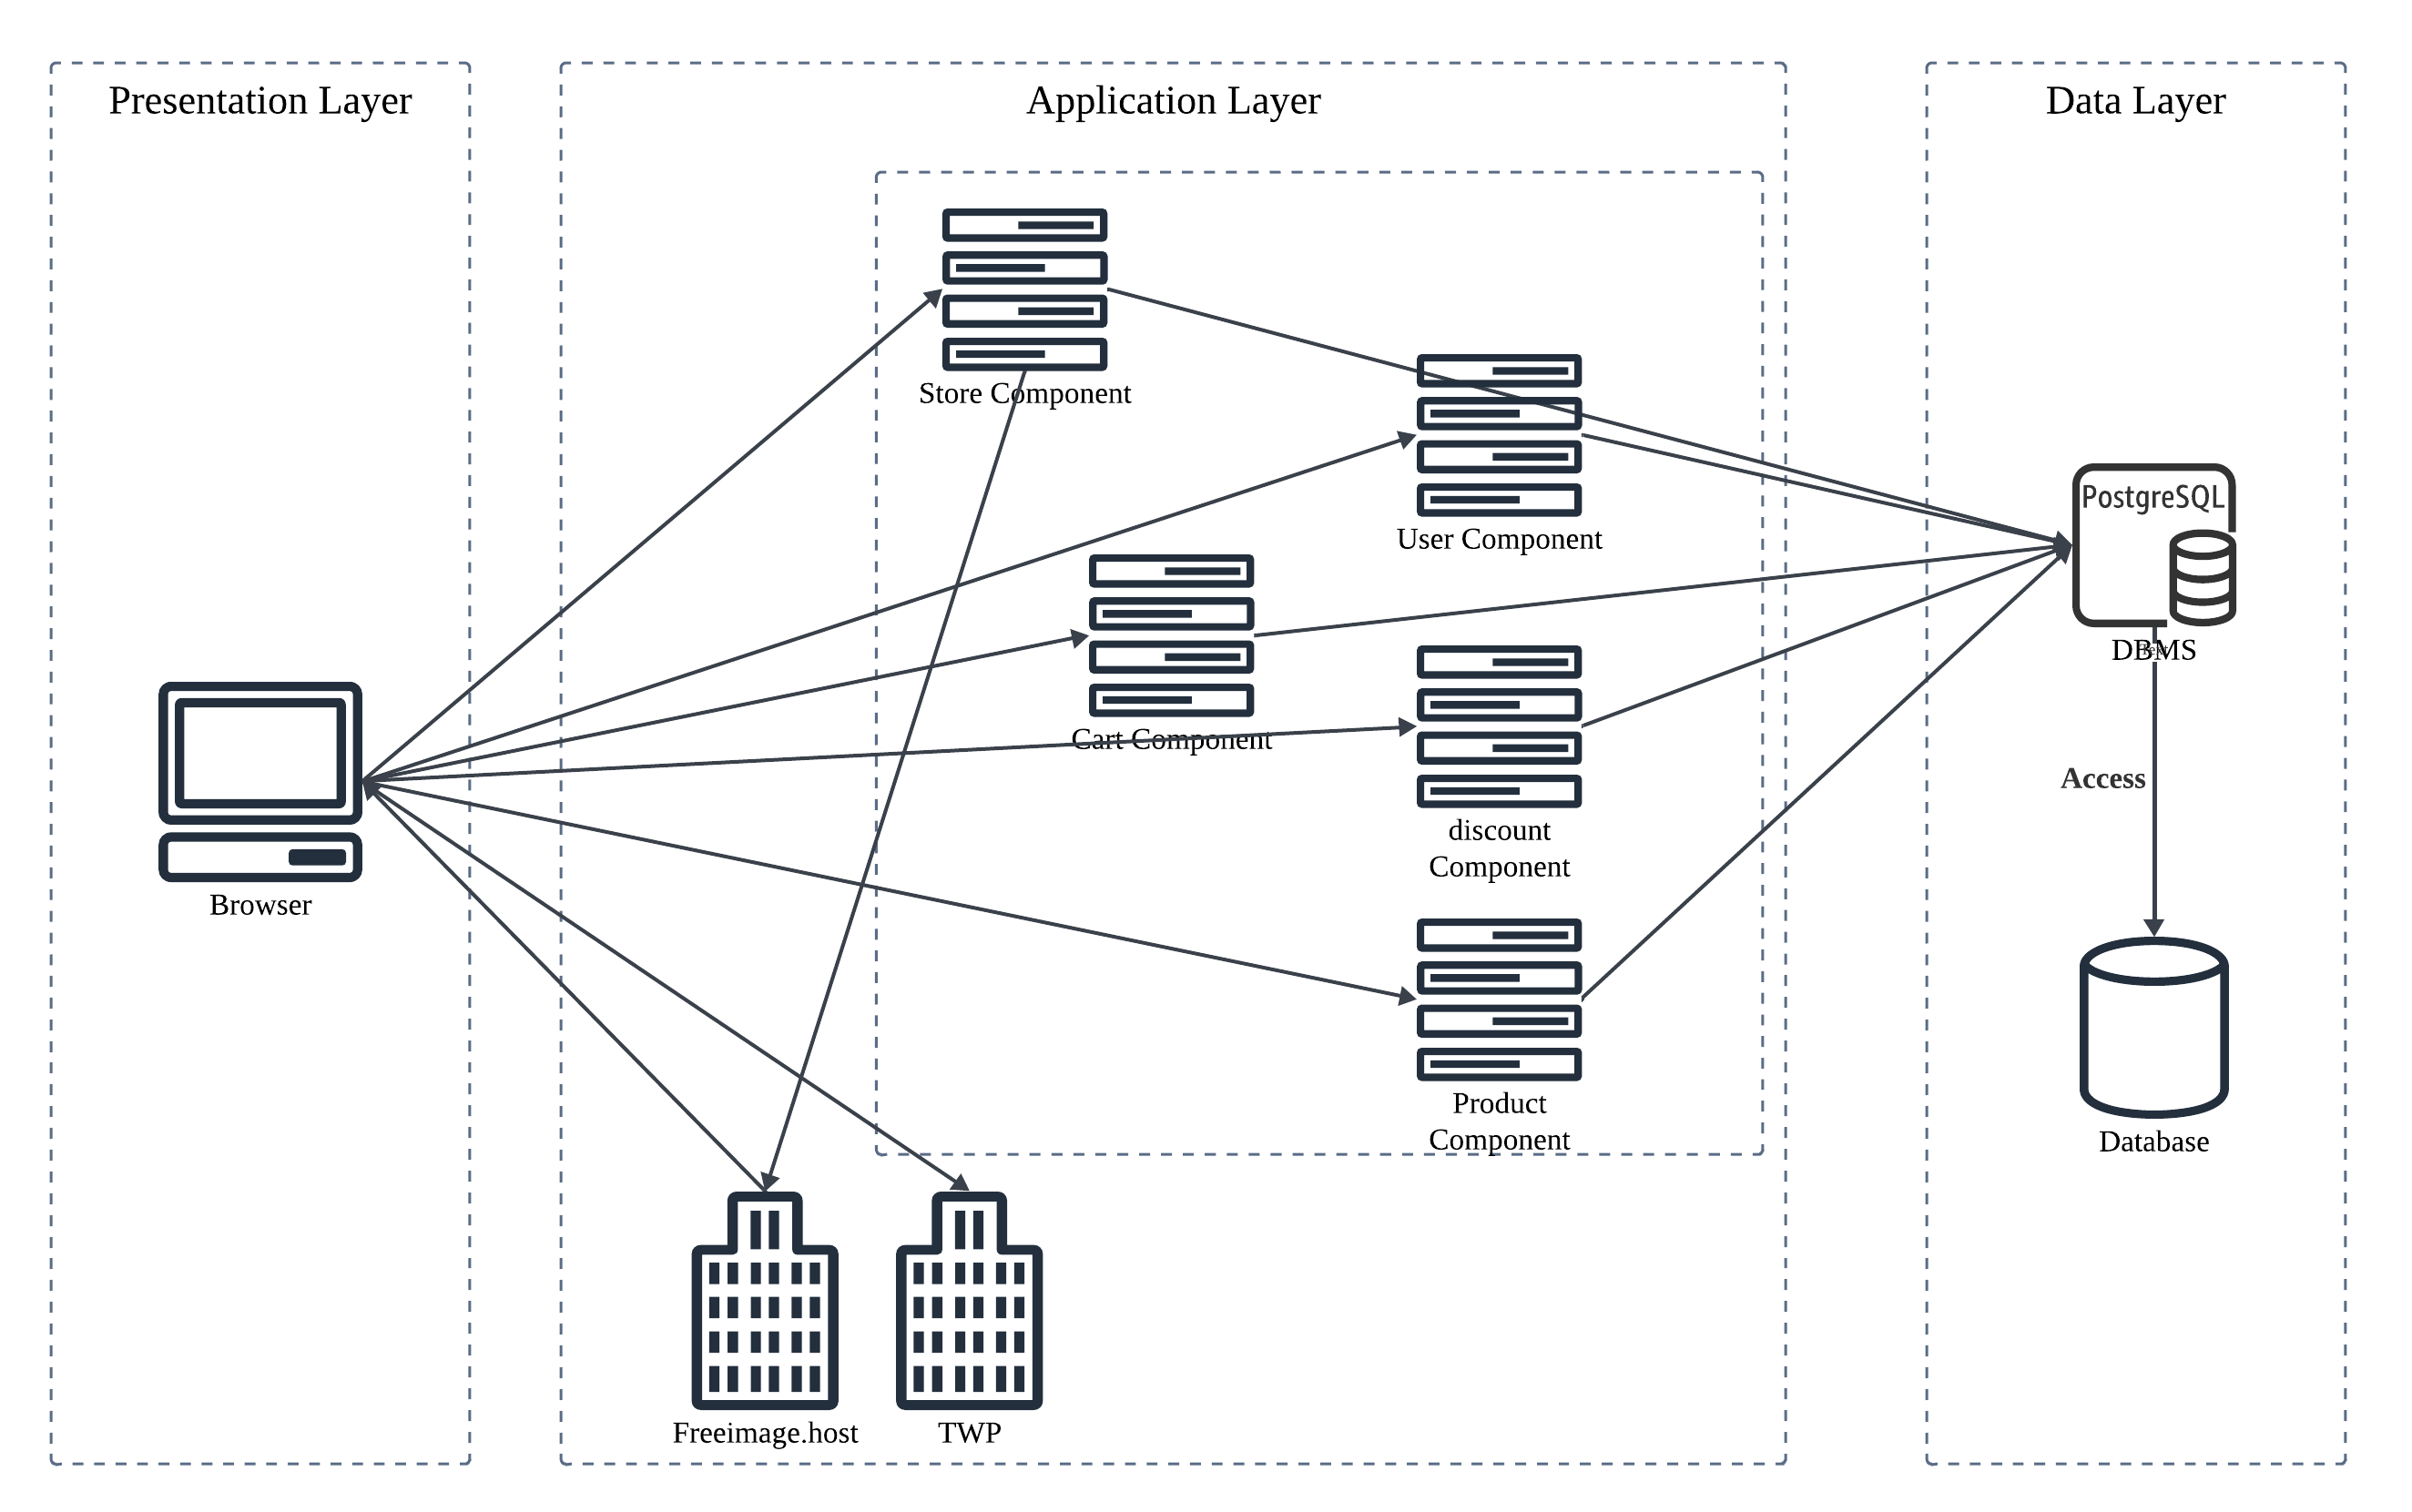
\includegraphics[width=31em]{System-Architecture-Diagram.png}
    \label{fig:enter-label}
\end{figure*}

\begin{figure*}[h]
    \centering
    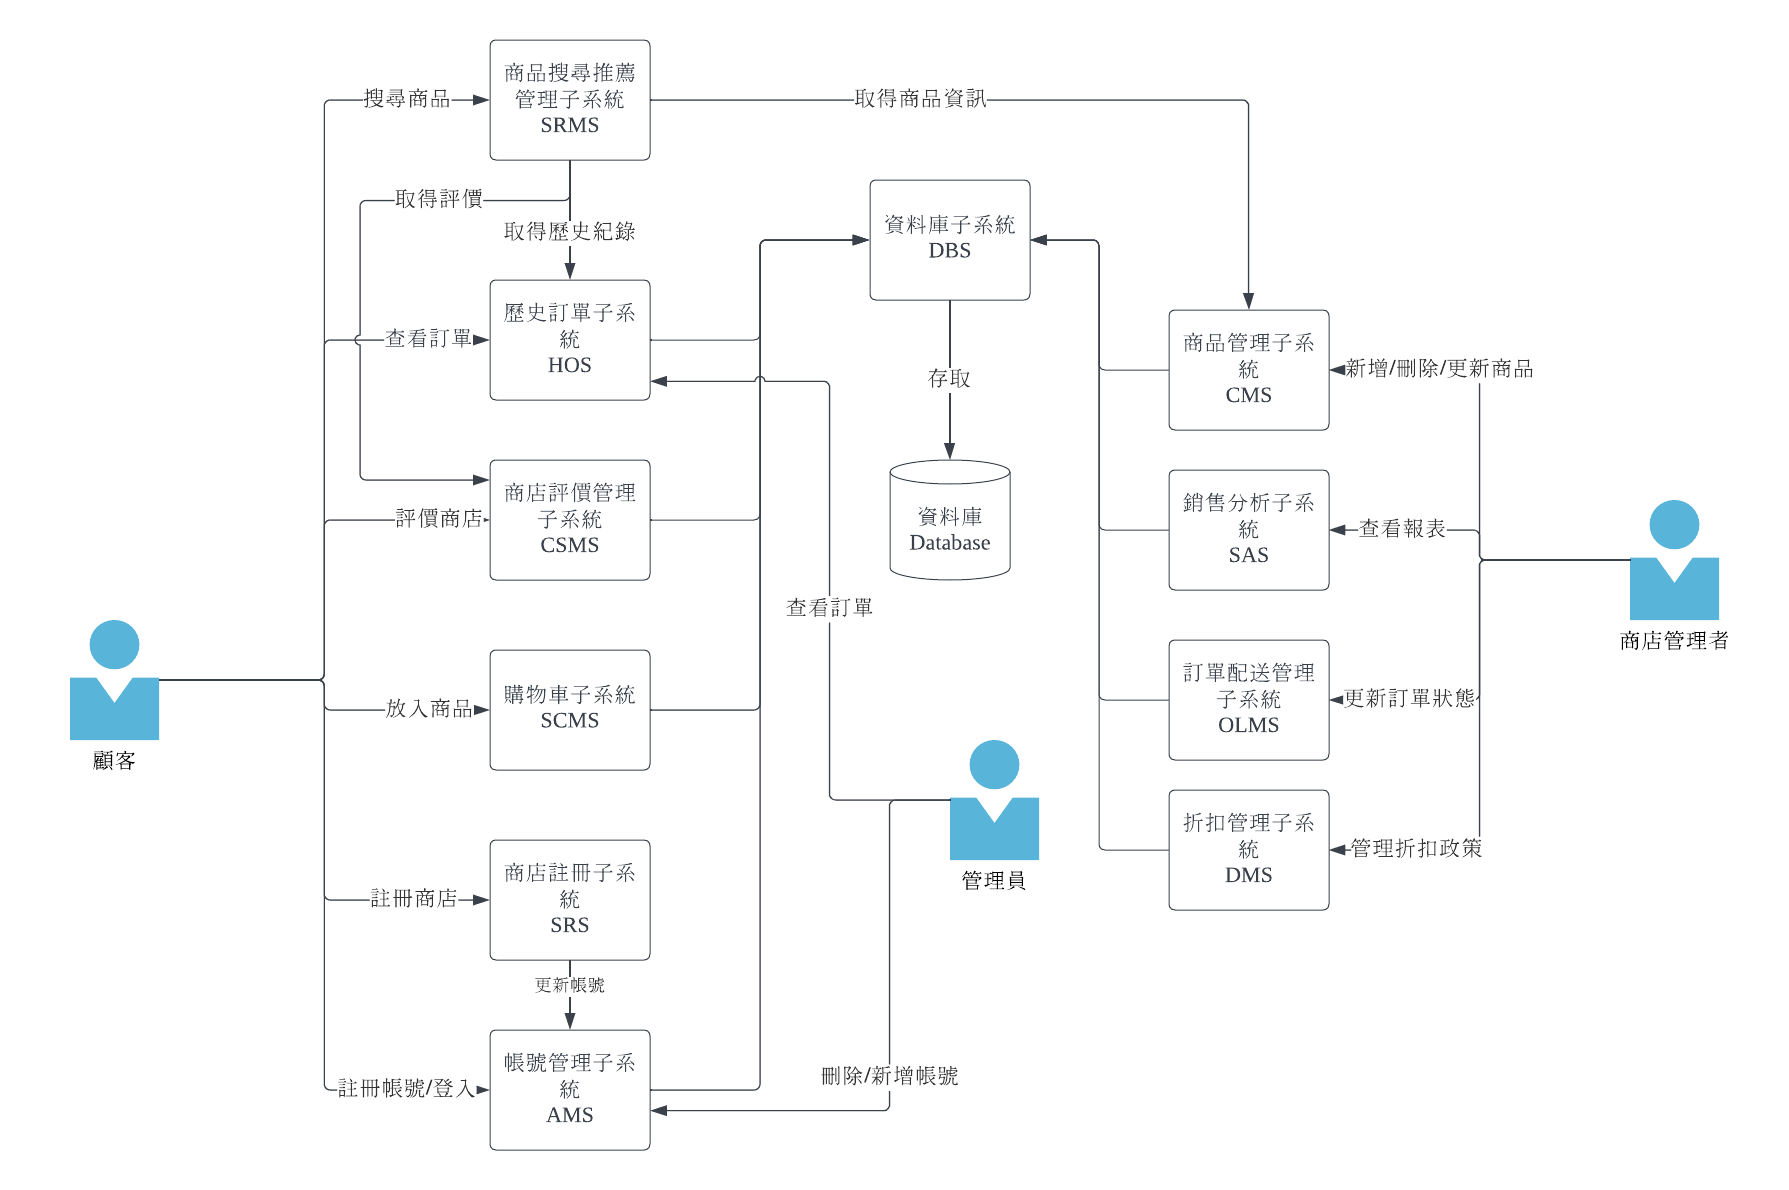
\includegraphics[width=30em]{System-Architecture-Diagram2.png}
    \label{fig:enter-label}
\end{figure*}
%\cite{aws_arch_diagram}
\newpage

\subsection{操作概念 (Operational Concepts or User Stories)}
\begin{itemize}
 
\item 顧客操作概念: \\
\setlength{\parindent}{2em} 使用者可以透過帳號管理子系統(AMS)進行註冊,用商品搜尋推薦管理子系統(SRMS)尋找自己想要的商品,透過歷史訂單子系統(HOS)查詢自己的訂單歷史紀錄,並透過購物車子系統(SCMS)將商品放入購物車並購買商品。
\item 商店管理者操作概念: \\
\setlength{\parindent}{2em} 顧客可以透過商店註冊系統(SRS)進行註冊成為商店管理者,用商品管理子系統(CMS)管理商品,用銷售分析子系統(SAS)產生財務報表,並透過訂單配送管理子系統(OLMS)管理顧客訂單。
\item 管理員操作概念: \\
\setlength{\parindent}{2em} 管理員可以透過帳號管理子系統(AMS)管理所有帳號,透過歷史訂單子系統(HOS)查看所有訂單紀錄。

\end{itemize}

% glu
\subsection{功能性需求 (Functional Requirements)}

\noindent \begin{tabular}{ | p{6.5em} | p{32em} |}
  \hline
  Notation & Description \\
  \hline
  WOS-F-001 & 顧客可以註冊帳號。 \\
  \hline
  WOS-F-002 & 顧客可以搜尋商店及商品。 \\
  \hline
  WOS-F-003 & 顧客可以將商品加入購物車。 \\
  \hline
  WOS-F-004 & 顧客可以結帳購物車內的商品。 \\
  \hline
  WOS-F-005 & 顧客可以查詢訂單狀態。 \\
  \hline
  WOS-F-006 & 顧客可以在訂單完成後為商店或商品評分。 \\
  \hline
  WOS-F-007 & 顧客可以查詢訂購歷史。 \\
  \hline
  WOS-F-008 & 顧客可以註冊商店成為商店管理員。 \\
  \hline
  WOS-F-009 & 商店管理者可以增加、刪減商品品項及數量。 \\
  \hline
  WOS-F-010 & 商店管理者可以查詢日、周、月銷售量及金額。 \\
  \hline
  WOS-F-011 & 商店管理者可以更新訂單狀況。 \\
  \hline
  WOS-F-012 & 商店管理者可以查詢、增加及刪減各項折扣方案。 \\
  \hline
  WOS-F-013 & 管理員可以新增、刪除、更新帳號。 \\
  \hline
  WOS-F-014 & 管理員可以查看所有訂單。 \\
  \hline
\end{tabular} \par

% lethe
\subsection{資料需求 (Data Requirements)}
\noindent\begin{tabular}{|l| p{32em}|}
    \hline
    需求編號 & 需求描述 \\
    \hline
    WOS-D-001 & 系統需儲存使用者的相關資訊:登入ID、姓名、密碼、電子郵件、地址 \\
    \hline
    WOS-D-002 & 系統需儲存產品的相關資訊:產品ID、名稱描述、其他屬性、產品圖片、價格、庫存產品數量、標籤 \\
    \hline
    WOS-D-003 & 系統需儲存商店的相關資訊:商店ID、名稱、地址、聯絡電子郵件、電話 \\
    \hline
    WOS-D-004 & 系統需儲存訂單的相關資訊:訂單ID、時間、客戶、每個採購項目的名稱和價格、每個採購項目的數量、採購總額、訂單的當前狀態(已接收、處理、運輸、關閉) \\
    \hline
    WOS-D-005 & 系統需儲存銷售報告的相關資訊:日期、商店名稱、訂單數量、銷售總額 \\
    \hline
\end{tabular}

% glu
\subsection{非功能性需求 (Non-Functional Requirements)}
\subsubsection{效能需求 (Performance Requirements)}
\noindent\begin{tabular}{|l| p{32em}|}
    \hline
    需求編號 & 需求描述 \\
    \hline
    WOS-N-001 & 網頁載入時間需不超過五秒 \\
    \hline
    WOS-N-002 & 用戶搜尋時間需不超過五秒 \\
    \hline
    WOS-N-003 & 商店管理員更新訂單及商店狀況至用戶端反映需不超過三十秒 \\
    \hline
\end{tabular}
\subsubsection{資安需求 (Security Requirements)}
\noindent\begin{tabular}{ | p{6.5em} | p{32em} |}
    \hline
    需求編號 & 需求描述 \\
    \hline
    WOS-N-004 & 註冊密碼必須符合複雜度需求 \\
    \hline
    WOS-N-005 & 管理員應遵守隱私權保護政策,不可隨意檢視個人資料 \\
    \hline
\end{tabular}
\subsection{介面需求 (Interface Requirements)}
% orange
\subsubsection{使用者介面需求 (User Interfaces Requirements)}
\setlength{\parindent}{2em} 買家介面
\begin{center}
\noindent\begin{tabular}{ | p{6.5em} | p{32em} |}
    \hline
    需求編號 & 需求描述 \\ 
    \hline
    WOS-I-001 & 搜尋食物or店家種類介面。\\
    \hline
    WOS-I-002 & 購物清單介面\\
    \hline
    WOS-I-003 & 點餐介面。\\
    \hline
    WOS-I-004 & 訂單配送管理界面。\\
    \hline
    \end{tabular}
\end{center}

\setlength{\parindent}{2em} 商家介面
\begin{center}
\noindent\begin{tabular}{ | p{6.5em} | p{32em} |}
    \hline
    需求編號 & 需求描述 \\ 
    \hline
    WOS-I-005 & 刊登商品資訊。\\
    \hline
    WOS-I-006 & 檢視買家訂單\\
    \hline
    WOS-I-007 & 管理刊登商品介面。\\
    \hline
    WOS-I-008 & 折扣管理介面。\\
    \hline
    WOS-I-009 & 檢視銷售報表介面。\\
    \hline
    \end{tabular}
\end{center}
    
\subsubsection{內部介面需求 (Internal Interface Requirements)}
\begin{center}
    \begin{tabular}{ | p{6.5em} | p{32em} |}
    \hline
    需求編號 & 需求描述 \\ 
    \hline
    WOS-I-010 & SRMS能向CMS接收商品資訊需求。\\
    \hline
    WOS-I-011 & SRMS能向HOS接收歷史訂單需求。\\
    \hline
    WOS-I-012 & SRMS能向CSMS接收評價需求。\\
    \hline
    WOS-I-013 & HOS與DBS需有傳送與接收歷史訂單需求。\\
    \hline
    WOS-I-014 & CSMS與DBS需有傳送與接收商店評價需求。\\
    \hline
    WOS-I-015 & SCMS與DBS需有傳送與接收購物車相關資訊需求。\\
    \hline
    WOS-I-016 & SRS能向AMS傳送更新帳號的需求。\\
    \hline
    WOS-I-017 & AMS與DBS需有傳送與接收帳號資訊需求。\\
    \hline
    WOS-I-018 & CMS與DBS需有傳送與接收商品資訊的需求。\\
    \hline
    WOS-I-019 & SAS能向DBS傳送取得銷售分析需求。\\
    \hline
    WOS-I-020 & OLMS能向DBS傳送更新訂單需求。\\
    \hline
    WOS-I-021 & DMS與DBS需有傳送與接收優惠資訊需求。\\
    \hline
    \end{tabular}
\end{center}
% wj4wj4
\subsection{其他需求 (Other Requirements)}
\subsubsection{環境需求 (Environmental Requirement)}
\begin{center}
    \begin{tabular}{ | p{6.5em} | p{32em} |}
    \hline
    需求編號 & 需求說明 \\ 
    \hline
    WOS-O-001 & 需要網路\\ 
    \hline
    WOS-O-002 & docker\\ 
    \hline
    WOS-O-003 & 中子\\ 
    \hline
    WOS-O-004 & 電子\\ 
    \hline
    WOS-O-005 & 質子(不會離開原子)\\ 
    \hline
    \end{tabular}
\end{center}
\subsubsection{安裝需求 (Installation Requirement)}
\begin{center}
    \begin{tabular}{ | p{6.5em} | p{32em} |}
    \hline
    需求編號 & 需求說明 \\ 
    \hline
    WOS-O-006 & 使用docker compose自動建置\\ 
    \hline
    \end{tabular}
\end{center}

\subsubsection{測試需求 (Test Requirements)}
\begin{center}
    \begin{tabular}{ | p{6.5em} | p{32em} |}
    \hline
    需求編號 & 需求說明 \\ 
    \hline
    WOS-O-007 & 所有子系統都應經過測試且無問題\\ 
    \hline
    \end{tabular}
\end{center}

\subsection{商業規則與限制 (Business Rules and Integrity Constrains)}

\noindent\begin{tabular}{ | p{6.5em} | p{32em} |}
\hline
需求編號 & 需求說明 \\ 
\hline
WOS-B-001 & 同一次購買可以應用三種類型的折扣,包括運費季節和特別活動折扣。\\
\hline
WOS-B-002 & 一種產品不能與多種特殊活動類型的折扣相關聯\\
\hline
WOS-B-003 & 產品的同一特殊活動折扣期間不能重疊。\\
\hline
WOS-B-004 & 購買的產品的數量必須是大於零的整數。\\
\hline
WOS-B-005 & 採購數量必須小於或等於該產品的當前庫存數量    \\
\hline
WOS-B-006 & 使用者可以有多個身份 \\
\hline
WOS-B-007 & 資料庫初始狀態要有所有員工和系統管理員的資訊 \\
\hline
\end{tabular}

\newpage

\section{Conceptual Design of the Database}
\subsection{Entity Relationship ER Model}

\begin{figure*}[h]
    \centerline{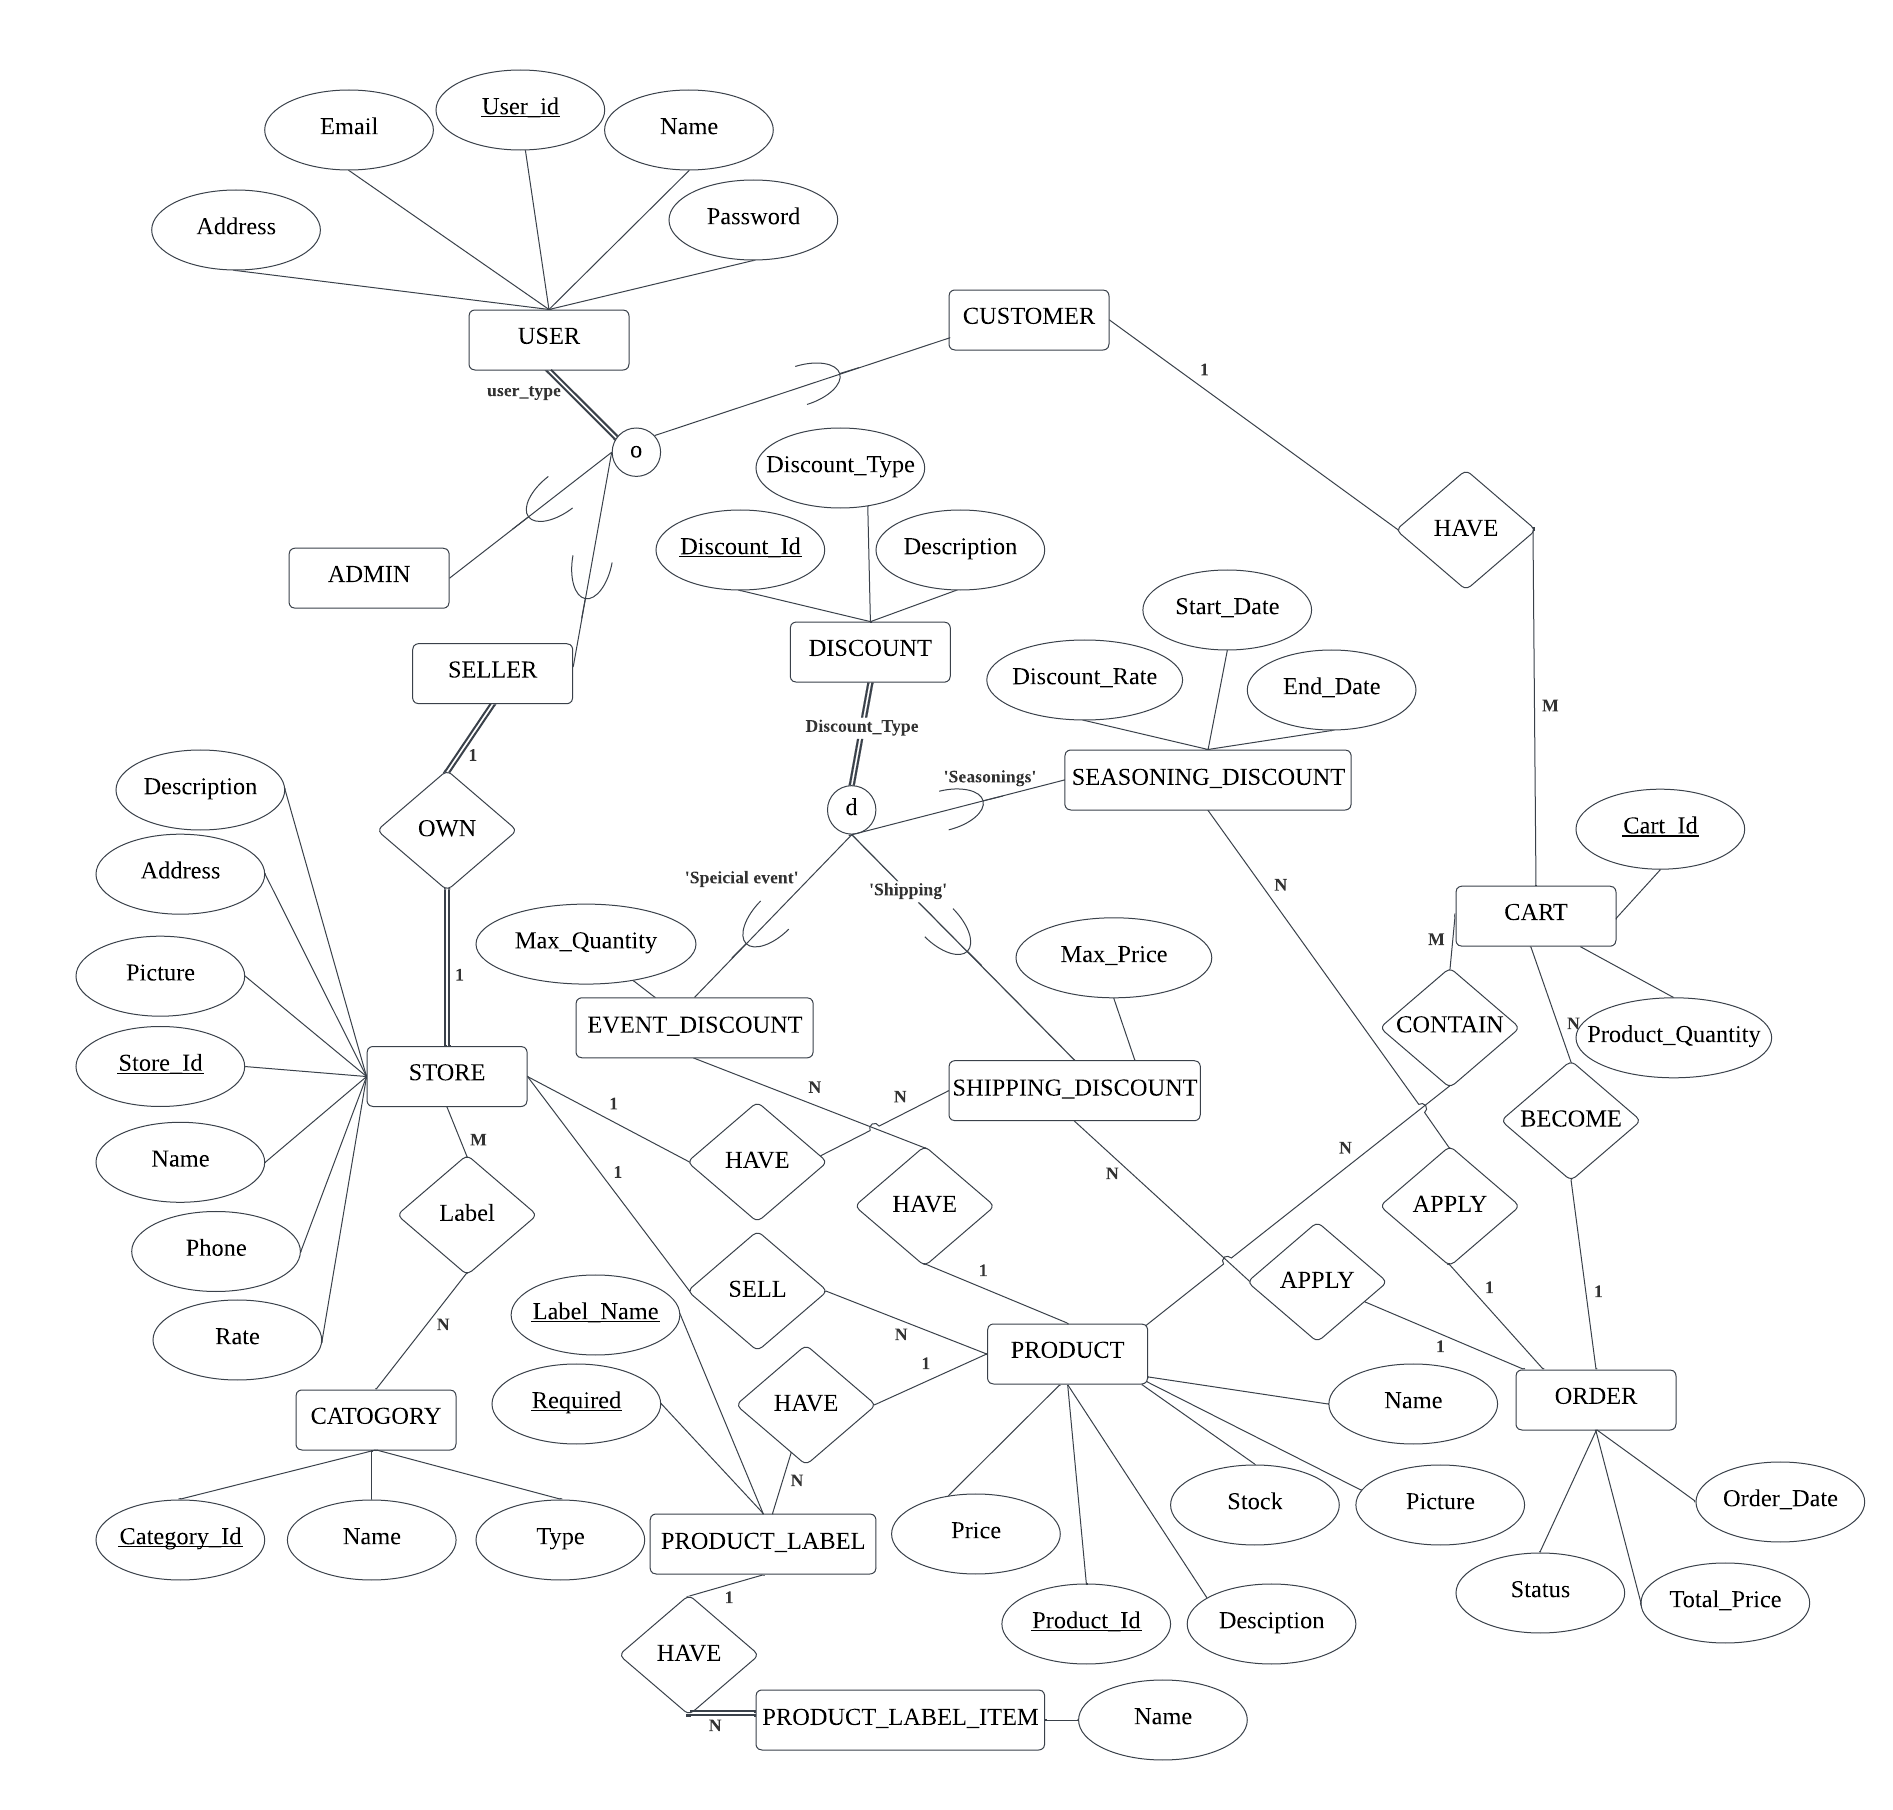
\includegraphics[width=40em]{ER-diagram.png}}
    \caption{ER diagram}
    \label{fig:enter-label}
\end{figure*}

\newpage

\subsection{Data Dictionary}
%User
\noindent\begin{tabular}{ | p{7em} | p{5.5em} |p{5.5em} | p{4.5em} | p{11em} |}
  \hline
  \multicolumn{5}{|c|}{USER_DATA} \tabularnewline
  \hline 
  \multicolumn{5}{|c|}{Description: 使用者相關資料} \tabularnewline
  \hline 
  Attribute & Type & Key & Nullable & Description \\
  \hline
  user_id & SERIAL & Primary & Not Null & 使用者ID \\
  \hline
  name & VARCHAR & &Not Null &使用者名稱\\
  \hline
  email & VARCHAR & &Not Null &使用者信箱\\
  \hline
  address & VARCHAR & &Not Null &使用者地址\\
  \hline
  password & VARCHAR & &Not Null &使用者密碼\\
  \hline
  authority & INTEGER & &Not Null&\makecell[l]{使用者權限\\(admin, seller, user)} \\
  \hline
  phone_number & VARCHAR & &Not Null &使用者電話號碼\\
  \hline
  current_cart_id & INTEGER & &Not Null &使用者目前購物車\\
  \hline
  status & INTEGER & & Not Null & \makecell[l]{使用者狀態\\(0=停用, 1=啟用)}\\
  \hline
  birthday & DATE & & Not Null &使用者生日\\
  \hline
\end{tabular}
\vspace{1em}

%Cart
\noindent\begin{tabular}{ | p{7em} | p{5.5em} |p{5.5em} | p{4.5em} | p{11em} |}
  \hline
  \multicolumn{5}{|c|}{CARTS} \tabularnewline
  \hline 
  \multicolumn{5}{|c|}{Description: 購物車相關資料} \tabularnewline
  \hline 
  Attribute & Type & Key & Nullable & Description \\
  \hline
  customer_id& SERIAL & \makecell[l]{Primary \\ Foreign}  & Not Null & 使用者ID \\
  \hline
  product_id & SERIAL &\makecell[l]{Primary \\ Foreign} &Not Null &商品ID\\
  \hline
  cart_id & INTEGER &\makecell[l]{Primary}  &Not Null &購物車ID\\
  \hline
  product_quantity & INTEGER & &Not Null &商品數量\\
  \hline
  event_discount_id & SERIAL & Foreign &Not Null &折價券ID\\
  \hline
  store_id & SERIAL & \makecell[l]{Primary\\ Foreign} & Not Null & 購買商店ID\\
  \hline
\end{tabular}
\vspace{1em}

% %Product
\noindent\begin{tabular}{ | p{7em} | p{5.5em} | p{5.5em} | p{4.5em} | p{11em} |}
  \hline
  \multicolumn{5}{|c|}{PRODUCTS} \tabularnewline
  \hline 
  \multicolumn{5}{|c|}{Description: 商品相關資料} \tabularnewline
  \hline 
  Attribute & Type & Key & Nullable & Description \\
  \hline
  product_id& SERIAL & \makecell[l]{Primary \\ Foreign}  & Not Null & 商品ID \\
  \hline
  name & VARCHAR & &Not Null &商品名字\\
  \hline
  description & TEXT & &Not Null &商品資訊\\
  \hline
  store_id & SERIAL &Foreign &Not Null &商店ID\\
  \hline
  picture & STRING & &Not Null &商品照片\\
  \hline
  price & INTEGER & &Not Null &商品價錢\\
  \hline
  stock & INTEGER &  &Not Null &商品庫存\\
  \hline
  status & INTEGER &  &Not Null &\makecell[l]{商品狀態\\(0=停用,\\ 1=啟用,\\ 2=已售完)}\\
  \hline
\end{tabular}
\vspace{1em}

% %Store
\noindent\begin{tabular}{ | p{7em} | p{5.5em} | p{5.5em} | p{4.5em} | p{11em} |}
  \hline
  \multicolumn{5}{|c|}{STORES} \tabularnewline
  \hline 
  \multicolumn{5}{|c|}{Description: 商店相關資料} \tabularnewline
  \hline 
  Attribute & Type & Key & Nullable & Description \\
  \hline
  store_id& SERIAL & Primary & Not Null & 商品ID \\
  \hline
  name & VARCHAR & &Not Null &商店名字\\
  \hline
  rate & FLOAT & &Not Null &商店評價\\
  \hline
  picture & STRING & &Not Null &商店照片\\
  \hline
  address & VARCHAR & &Not Null &商店地址\\
  \hline
  description & TEXT & &Not Null &商店描述\\
  \hline
  shipping_fee & INTEGER & &Not Null &運費\\
  \hline
  status & INTEGER & &Not Null &\makecell[l]{商店狀態\\(0=停用, 1=啟用)}\\
  \hline
  rate_count & INTEGER & &Not Null &評價數量\\
  \hline
\end{tabular}
\vspace{1em}

%Label
\noindent\begin{tabular}{ | p{7em} | p{5.5em} | p{5.5em} | p{4.5em} | p{11em} |}
  \hline
  \multicolumn{5}{|c|}{LABEL} \tabularnewline
  \hline 
  \multicolumn{5}{|c|}{Description: 商店標籤資料} \tabularnewline
  \hline 
  Attribute & Type & Key & Nullable & Description \\
  \hline
  store_id& SERIAL & \makecell[l]{Primary \\ Foreign}& Not Null & 商店ID \\
  \hline
  category_id & SERIAL & \makecell[l]{Primary \\ Foreign} &Not Null &目錄ID\\
  \hline
\end{tabular}
\vspace{1em}

%Categories
\noindent\begin{tabular}{ | p{7em} | p{5.5em} | p{5.5em} | p{4.5em} | p{11em} |}
  \hline
  \multicolumn{5}{|c|}{CATEGORIES} \tabularnewline
  \hline 
  \multicolumn{5}{|c|}{Description: 類別資料} \tabularnewline
  \hline 
  Attribute & Type & Key & Nullable & Description \\
  \hline
  category_id& SERIAL & Primary & Not Null & 類別ID \\
  \hline
  name & VARCHAR & &Not Null &類別名稱\\
  \hline
\end{tabular}

\vspace{1em}
%enent_discount
\noindent\begin{tabular}{ | p{7em} | p{5.5em} | p{5.5em} | p{4.5em} | p{11em} |}
  \hline
  \multicolumn{5}{|c|}{EVENT_DISCOUNT} \tabularnewline
  \hline 
  \multicolumn{5}{|c|}{Description: 事件折扣資料} \tabularnewline
  \hline 
  Attribute & Type & Key & Nullable & Description \\
  \hline
  discount_id & SERIAL & Primary & Not Null & 折扣ID \\
  \hline
  max_quantity & INTEGER & &Not Null &買x送一\\
  \hline
  product_id & SERIAL & Foreign &Not Null &商品ID\\
  \hline
\end{tabular}
\vspace{1em}

%Shipping_discount
\noindent\begin{tabular}{ | p{7em} | p{5.5em} | p{5.5em} | p{4.5em} | p{11em} |}
  \hline
  \multicolumn{5}{|c|}{SHIPPING_DISCOUNT} \tabularnewline
  \hline 
  \multicolumn{5}{|c|}{Description: 運費折扣資料} \tabularnewline
  \hline 
  Attribute & Type & Key & Nullable & Description \\
  \hline
  discount_id & SERIAL & Primary & Not Null & 折扣ID \\
  \hline
  max_price & INTEGER & &Not Null &免運金額\\
  \hline
  store_id & SERIAL & Foreign &Not Null &商店ID\\
  \hline
\end{tabular}
\vspace{1em}

%Discount
\noindent\begin{tabular}{ | p{7em} | p{5.5em} | p{5.5em} | p{4.5em} | p{11em} |}
  \hline
  \multicolumn{5}{|c|}{DISCOUNTS} \tabularnewline
  \hline 
  \multicolumn{5}{|c|}{Description: 折扣資料} \tabularnewline
  \hline 
  Attribute & Type & Key & Nullable & Description \\
  \hline
  discount_id & SERIAL & Primary & Not Null & \makecell[l]{折扣ID\\1=無折扣} \\
  \hline
  discount_type & INTEGER &  & Not Null & \makecell[l]{折扣種類\\0=無折扣\\1=運費折扣\\2=季節性折扣\\3=事件折扣} \\
  \hline
  status & INTEGER & &Not Null &狀態\\
  \hline
  description& VARCHAR &  &Not Null &折價資訊\\
  \hline
  name & VARCHAR &  &Not Null &折扣名稱\\
  \hline
\end{tabular}
\vspace{1em}

%Order
\noindent\begin{tabular}{ | p{7em} | p{5.5em} | p{5.5em} | p{4.5em} | p{11em} |}
  \hline
  \multicolumn{5}{|c|}{ORDER} \tabularnewline
  \hline 
  \multicolumn{5}{|c|}{Description: 訂單} \tabularnewline
  \hline 
  Attribute & Type & Key & Nullable & Description \\
  \hline
  order_date & DATE &  & Not Null & 訂單日期 \\
  \hline
  total_price & INTEGER &  & Not Null & 總金額 \\
  \hline
  seasoning_discount_id & SERIAL & Foreign&Not Null &季節折扣ID\\
  \hline
  shipping_discount_id & SERIAL & Foreign&Not Null &運費折扣ID\\
  \hline
  cart_id& SERIAL & \makecell[l]{Primary \\ Foreign} &Not Null &購物車ID\\
  \hline
  customer_id & SERIAL & \makecell[l]{Primary \\ Foreign} & Not Null & 顧客ID \\
  \hline
  taking_method & INTEGER &  & Not Null &  \makecell[l]{0=自取\\1=外送}\\
  \hline
  store_id & SERIAL & \makecell[l]{Primary \\ Foreign} & Not Null & 商店ID \\
  \hline
  taking_address & VARCHAR &  & Not Null & 運送地址 \\
  \hline
  status & INTEGER &  & Not Null & \makecell[l]{訂單狀態\\0=未結帳\\1=已結帳\\2=接受訂單\\3=製作訂單\\4=運送中\\5=已送達\\6=確認訂單\\7=已評分} \\
  \hline
\end{tabular}


%Seasoning_discount
\noindent\begin{tabular}{ | p{7em} | p{5.5em} | p{5.5em} | p{4.5em} | p{11em} |}
  \hline
  \multicolumn{5}{|c|}{SEASONING_DISCOUNT} \tabularnewline
  \hline 
  \multicolumn{5}{|c|}{Description: 季節折扣資料} \tabularnewline
  \hline 
  Attribute & Type & Key & Nullable & Description \\
  \hline
  discount_id & SERIAL & Primary & Not Null & 折扣ID \\
  \hline
  start_date & DATE &  & Not Null & 開始日期 \\
  \hline
  end_date & DATE & &Not Null &結束日期\\
  \hline
  store_id& SERIAL & Foreign &Not Null &商店ID\\
  \hline
  discount_percentage & INTEGER &  &Not Null &\makecell[l]{折扣比例\\(70=30\%off)}\\
  \hline
\end{tabular}

%product_label
\noindent\begin{tabular}{ | p{7em} | p{5.5em} | p{5.5em} | p{4.5em} | p{11em} |}
  \hline
  \multicolumn{5}{|c|}{PRODUCT_LABEL} \tabularnewline
  \hline 
  \multicolumn{5}{|c|}{Description: 商品標籤} \tabularnewline
  \hline 
  Attribute & Type & Key & Nullable & Description \\
  \hline
  product_id & SERIAL & \makecell[l]{Primary \\ Foreign} & Not Null & 商品ID \\
  \hline
  label_name & VARCHAR & \makecell[l]{Primary \\ Foreign} & Not Null & 類別名稱 \\
  \hline
  required & BOOLEAN & & Not Null & 是否為必填\\
  \hline
\end{tabular}

%product_label_item
\noindent\begin{tabular}{ | p{7em} | p{5.5em} | p{5.5em} | p{4.5em} | p{11em} |}
  \hline
  \multicolumn{5}{|c|}{PRODUCT_LABEL_ITEM} \tabularnewline
  \hline 
  \multicolumn{5}{|c|}{Description: 商品標籤選項} \tabularnewline
  \hline 
  Attribute & Type & Key & Nullable & Description \\
  \hline
  product_id & SERIAL & \makecell[l]{Primary \\ Foreign} & Not Null & 商品ID \\
  \hline
  label_name & VARCHAR & \makecell[l]{Primary \\ Foreign} & Not Null & 類別名稱 \\
  \hline
  name & VARCHAR & Primary & Not Null & 選項名稱\\
  \hline
\end{tabular}

\newpage

\section{Logical Database Schema}
\subsection{Schema of the Database}

\begin{figure*}[h]
    \centerline{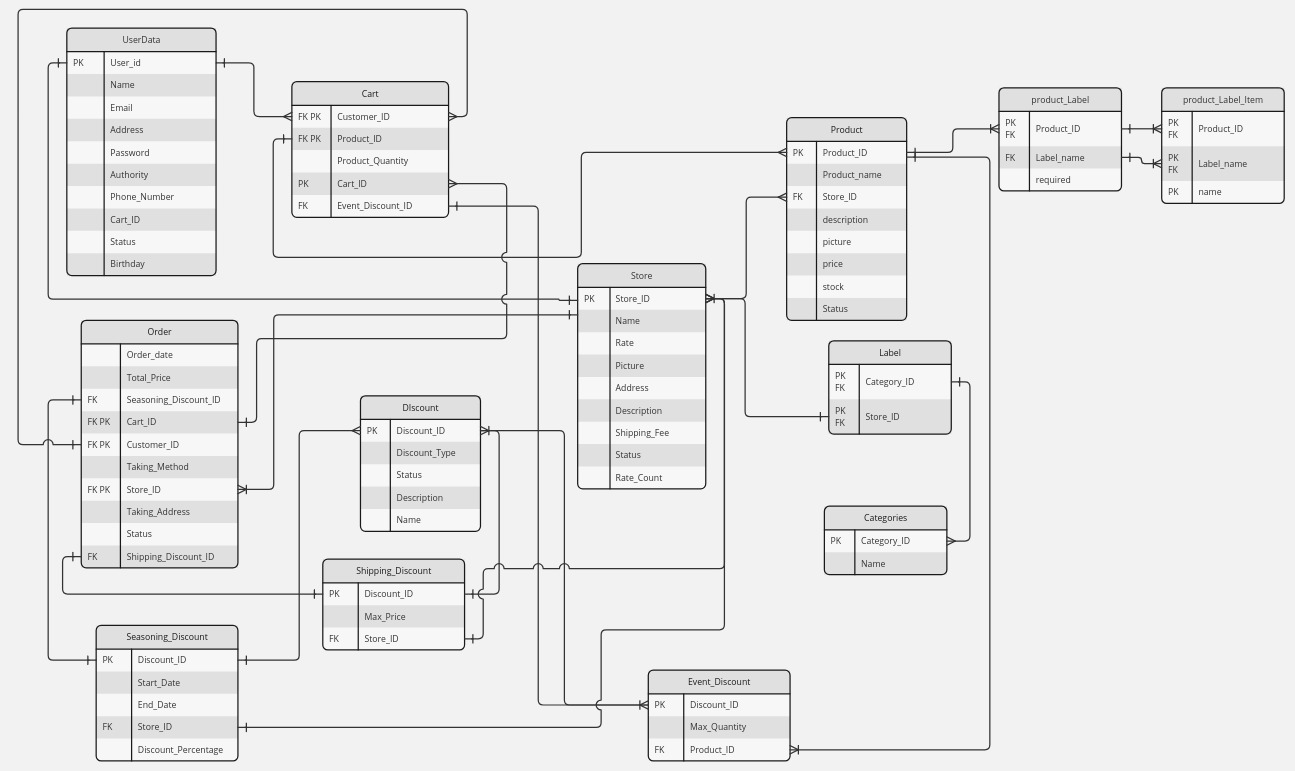
\includegraphics[width=40em]{schema-diagram.jpg}}    
    \caption{database schema}
    \label{fig:enter-label}
\end{figure*}

\newpage

\subsection{Snapshot of Tables}
\begin{figure}[hp]
    \centerline{\includegraphics[width=\linewidth]{snapshot/user_data.png}}
    \caption{user_data}
\end{figure}


\begin{figure}[hp]
    \centerline{\includegraphics[width=\linewidth]{snapshot/stores.png}}
    \caption{stores}
\end{figure}

\begin{figure}[hp]
    \centerline{\includegraphics[width=\linewidth]{snapshot/carts.png}}
    \caption{carts}
\end{figure}

\begin{figure}[hp]
    \centerline{\includegraphics[width=\linewidth]{snapshot/categories.png}}
    \caption{categories}
\end{figure}

\begin{figure}[hp]
    \centerline{\includegraphics[width=\linewidth]{snapshot/products.png}}
    \caption{products}
\end{figure}

\begin{figure}[hp]
    \centerline{\includegraphics[width=\linewidth]{snapshot/discounts.png}}
    \caption{discounts}
\end{figure}

\begin{figure}[hp]
    \centerline{\includegraphics[width=\linewidth]{snapshot/shipping_discount.png}}
    \caption{shipping_discount}
\end{figure}

\begin{figure}[hp]
    \centerline{\includegraphics[width=\linewidth]{snapshot/event_discount.png}}
    \caption{event_discount}
\end{figure}

\begin{figure}[hp]
    \centerline{\includegraphics[width=\linewidth]{snapshot/seasoning_discount.png}}
    \caption{seasoning_discount}
\end{figure}

\begin{figure}[hp]
    \centerline{\includegraphics[width=\linewidth]{snapshot/orders.png}}
    \caption{orders}
\end{figure}

\begin{figure}[hp]
    \centerline{\includegraphics[width=\linewidth]{snapshot/product_label.png}}
    \caption{product_label}
\end{figure}

\begin{figure}[hp]
    \centerline{\includegraphics[width=\linewidth]{snapshot/label_item.png}}
    \caption{label_item}
\end{figure}

\clearpage

\begin{figure}[h!]
    \centerline{\includegraphics[width=\linewidth]{snapshot/labels.png}}
    \caption{labels}
\end{figure}

\clearpage

\subsection{SQL Statements for Database Construction}
\subsubsection{Create Table}
\begin{lstlisting}
-- user_data
CREATE TABLE
    IF NOT EXISTS user_data(
        user_id SERIAL PRIMARY KEY,
        name VARCHAR(32) NOT NULL,
        password VARCHAR(32) NOT NULL,
        email VARCHAR(64) UNIQUE NOT NULL,
        address VARCHAR(64) NOT NULL,
        phone_number VARCHAR(16) NOT NULL,
        birthday DATE NOT NULL,
        authority INTEGER NOT NULL,
        current_cart_id INTEGER NOT NULL,
        status INTEGER NOT NULL
    );
\end{lstlisting}

\begin{lstlisting}
-- stores
CREATE TABLE
    IF NOT EXISTS stores (
        store_id SERIAL PRIMARY KEY REFERENCES user_data(user_id),
        name VARCHAR(255) NOT NULL,
        rate FLOAT NOT NULL,
        rate_count INTEGER NOT NULL,
        address VARCHAR(255) NOT NULL,
        picture VARCHAR(255) NOT NULL,
        description TEXT NOT NULL,
        shipping_fee INTEGER NOT NULL,
        status INTEGER NOT NULL
    );
\end{lstlisting}

\begin{lstlisting}
-- products
CREATE TABLE
    IF NOT EXISTS products (
        product_id SERIAL PRIMARY KEY,
        store_id SERIAL REFERENCES stores(store_id),
        name VARCHAR(255) NOT NULL,
        description TEXT NOT NULL,
        picture VARCHAR(255) NOT NULL,
        price INTEGER NOT NULL,
        stock INTEGER NOT NULL,
        status INTEGER NOT NULL
    );
\end{lstlisting}

\begin{lstlisting}
-- discounts
CREATE TABLE
    IF NOT EXISTS discounts (
        discount_id SERIAL PRIMARY KEY UNIQUE,
        discount_type INT NOT NULL,
        status INT NOT NULL,
        description TEXT,
        name VARCHAR(255) NOT NULL
    );
\end{lstlisting}

\begin{lstlisting}
-- seasoning_discount
CREATE TABLE
    IF NOT EXISTS seasoning_discount (
        discount_id SERIAL UNIQUE REFERENCES discounts(discount_id),
        discount_percentage INT NOT NULL,
        start_date DATE NOT NULL,
        end_date DATE NOT NULL
    );
\end{lstlisting}

\begin{lstlisting}
-- shopping_discount
CREATE TABLE
    IF NOT EXISTS shipping_discount (
        discount_id SERIAL UNIQUE REFERENCES discounts(discount_id),
        max_price INT NOT NULL,
        store_id SERIAL REFERENCES stores(store_id)
    );
\end{lstlisting}

\begin{lstlisting}
-- event_discount
CREATE TABLE
    IF NOT EXISTS event_discount (
        discount_id SERIAL UNIQUE REFERENCES discounts(discount_id),
        max_quantity INT NOT NULL,
        product_id SERIAL REFERENCES products(product_id)
    );
\end{lstlisting}

\begin{lstlisting}
-- carts
CREATE TABLE
    IF NOT EXISTS carts (
        customer_id SERIAL REFERENCES user_data(user_id),
        product_id SERIAL REFERENCES products(product_id),
        store_id SERIAL REFERENCES stores(store_id),
        cart_id INTEGER NOT NULL,
        product_quantity INT NOT NULL,
        event_discount_id SERIAL REFERENCES discounts(discount_id),
        PRIMARY KEY (
            customer_id,
            product_id,
            store_id,
            cart_id
        )
    );
\end{lstlisting}

\begin{lstlisting}
-- orders
CREATE TABLE
    orders (
        cart_id INTEGER,
        store_id INTEGER REFERENCES stores(store_id),
        user_id INTEGER REFERENCES user_data(user_id),
        seasoning_discount_id INTEGER REFERENCES discounts(discount_id),
        shipping_discount_id INTEGER REFERENCES discounts(discount_id),
        status INTEGER,
        total_price INTEGER,
        Order_date TIMESTAMP,
        taking_address VARCHAR(255),
        taking_method INTEGER,
        PRIMARY KEY (cart_id, store_id, user_id)
    );
\end{lstlisting}

\begin{lstlisting}
-- categories
CREATE TABLE
    IF NOT EXISTS categories (
        category_id SERIAL PRIMARY KEY,
        name VARCHAR(255) UNIQUE NOT NULL
    );
\end{lstlisting}

\begin{lstlisting}
-- product_label
CREATE TABLE
    IF NOT EXISTS product_label (
        product_id SERIAL REFERENCES products(product_id),
        label_name VARCHAR(255) NOT NULL,
        required BOOLEAN NOT NULL,
        PRIMARY KEY (product_id, label_name)
    );
\end{lstlisting}

\begin{lstlisting}
-- label_item
CREATE TABLE
    IF NOT EXISTS label_item (
        product_id SERIAL NOT NULL,
        label_name VARCHAR(255) NOT NULL,
        item_name VARCHAR(255) NOT NULL,
        FOREIGN KEY (product_id, label_name) REFERENCES product_label(product_id, label_name),
        PRIMARY KEY (product_id, label_name, item_name)
    );
\end{lstlisting}

\subsubsection{Insert Data}

\begin{lstlisting}
-- user_data
INSERT INTO user_data (name, password, email, address, phone_number, birthday, authority, current_cart_id, status) VALUES
    ('admin', 'admin', 'admin@gmail.com', 'address_admin', '0900-0000', '2021-10-10 11:30:30', 111, 1, 1),
    ('alice', 'pwd1', 'a@gmail.com', 'address_1', '0900-1111', '2021-10-10 11:30:30', 001, 1, 1),
    ('bob', 'pwd2', 'b@gmail.com', 'address_2', '0900-2222', '2022-11-11 11:30:30', 010, 2, 1),
    ('tcp', 'pwd3', 'c@gmail.com', 'address_3', '0900-3333', '2023-12-12 11:30:30', 001, 1, 1),
    ('udp', 'pwd4', 'd@gmail.com', 'address_4', '0900-4444', '2024-01-01 11:30:30', 011, 1, 1),
    ('icmp', 'pwd5', 'e@gmail.com', 'address_5', '0900-5555', '2025-02-02 11:30:30', 001, 1, 1),
    ('dns', 'pwd6', 'f@gmail.com', 'address_6', '0900-6666', '2026-03-03 11:30:30', 001, 1, 1),
    ('dhcp', 'pwd7', 'g@gmail.com', 'address_7', '0900-7777', '2027-04-04 11:30:30', 001, 1, 1);
\end{lstlisting}

\begin{lstlisting}
-- stores
INSERT INTO stores (store_id, name, rate, rate_count, address, picture, description, shipping_fee, status) VALUES 
    (1, 'im pasta', 4, 100, 'pun street', 'https://i.imgur.com/3i3tyXJ.gif', 'you are not pasta', 35, 1),
    (3, 'number five',3.5, 5, 'pun street', 'https://i.imgur.com/3i3tyXJ.gif', 'special meal', 15, 1),
    (2, 'mos burger',4, 123, 'NTUT', 'https://i.imgur.com/3i3tyXJ.gif', 'moooooooooooooos', 55, 1),
    (7, 'trash noodle',4.9, 9876, 'pun street', 'https://i.imgur.com/3i3tyXJ.gif', 'trash', 192, 1);
\end{lstlisting}

\begin{lstlisting}
-- products
INSERT INTO products (store_id, name, description, picture, price, stock, status) VALUES
    (1, 'pasta', 'tasty pasta', 'https://i.imgur.com/3i3tyXJ.gif', 150, 100, 1),
    (1, 'black tea', 'student card get free', 'https://i.imgur.com/3i3tyXJ.gif', 0, 100, 1),
    (2, 'special1', 'special', 'https://i.imgur.com/3i3tyXJ.gif', 250, 2, 1),
    (2, 'special2', 'special', 'https://i.imgur.com/3i3tyXJ.gif', 350, 2, 0),
    (2, 'special3', 'special', 'https://i.imgur.com/3i3tyXJ.gif', 450, 2, 1),
    (3, 'black tea', 'most famous', 'https://i.imgur.com/3i3tyXJ.gif', 300, 3, 1),
    (3, 'rice burger', 'we have rice', 'https://i.imgur.com/3i3tyXJ.gif', 500, 3, 2),
    (7, 'big trash', 'can add kimchi for free', 'https://i.imgur.com/3i3tyXJ.gif', 80, 3, 1),
    (7, 'small trash', 'can add kimchi for free', 'https://i.imgur.com/3i3tyXJ.gif', 60, 3, 1);
\end{lstlisting}

\begin{lstlisting}
-- discounts
INSERT INTO discounts (discount_type, description, name, status) VALUES
(0, 'no discount', 'default', 1),
(1, 'all products 90% off', 'spring discount', 1),
(1, 'all products 80% off', 'spring discount', 1),
(1, 'all products 70% off', 'spring discount', 1),
(2, 'free shipping when price over 1000', 'spring discount', 1),
(2, 'free shipping when price over 500', 'spring discount', 1),
(2, 'free shipping when price over 300', 'spring discount', 1),
(3, 'buy 3 get 1 free', 'halloween', 1),
(3, 'buy 2 get 1 free', 'halloween', 1),
(3, 'buy 1 get 1 free', 'halloween', 1);
\end{lstlisting}

\begin{lstlisting}
-- seasoning_discount
INSERT INTO seasoning_discount (discount_id, discount_percentage, start_date, end_date) VALUES
    (2,90,'2021-01-01 00:00:00','2021-01-02 00:00:00'),
    (3,80,'2021-01-03 00:00:00','2021-01-04 00:00:00'),
    (4,70,'2021-01-05 00:00:00','2021-01-05 00:00:00');
\end{lstlisting}

\begin{lstlisting}
-- shipping_discount
INSERT INTO shipping_discount (discount_id, max_price, store_id) VALUES
  (5,1000,1),
  (6,500,1),
  (7,300,1);
\end{lstlisting}

\begin{lstlisting}
-- event_discount
INSERT INTO event_discount (discount_id, max_quantity, product_id) VALUES
    (8,3,1),
    (9,3,2),
    (10,3,3);
\end{lstlisting}

\begin{lstlisting}
-- carts
INSERT INTO carts (customer_id, cart_id, store_id, product_id, product_quantity, event_discount_id) VALUES
    (1, 1, 1, 2, 100, 8),
    (1, 1, 1, 1, 100, 9),
    (1, 2, 1, 2, 33, 10),
    (3, 1, 2, 3, 100, 1),
    (1, 3, 1, 1, 7, 1);
\end{lstlisting}

\begin{lstlisting}
-- orders
INSERT INTO orders (user_id, cart_id, store_id, seasoning_discount_id, shipping_discount_id, status, total_price, Order_date, taking_address, taking_method) VALUES 
    (1, 1, 1, 1, 1, 1, 100, '2020-01-01 00:00:00', '台北市', 1),
    (1, 2, 1, 2, 5, 1, 100, '2020-02-01 00:00:00', '台北市', 1),
    (3, 1, 2, 3, 6, 1, 100, '2020-03-01 00:00:00', '台北市', 1),
    (1, 3, 1, 4, 7, 1, 100, '2020-04-01 00:00:00', '台北市', 1);
\end{lstlisting}

\begin{lstlisting}
-- categories
INSERT INTO categories (name) VALUES
    ('Spices'),
    ('Sustainable'),
    ('Fresh'),
    ('Bakery'),
    ('Local'),
    ('sus thing');
\end{lstlisting}

\begin{lstlisting}
-- labels
INSERT INTO labels (category_id, store_id) VALUES
    (1, 1),
    (2, 1),
    (3, 1),
    (2, 2),
    (5, 7),
    (6, 7);
\end{lstlisting}

\begin{lstlisting}
-- product_label
INSERT INTO product_label (product_id, label_name, required) VALUES
    (2,'sugar', true),
    (7,'rice', true),
    (8, 'kimchi', false),
    (9, 'kimchi', false);
\end{lstlisting}

\begin{lstlisting}
-- label_item
INSERT INTO label_item (product_id, label_name, item_name) VALUES
    (2, 'sugar', 'more'),
    (2, 'sugar', 'less'),
    (2, 'sugar', 'no'),
    (7, 'rice', 'yes'),
    (7, 'rice', 'no'),
    (8, 'kimchi', 'yes'),
    (8, 'kimchi', 'no'),
    (9, 'kimchi', 'yes'),
    (9, 'kimchi', 'no');
\end{lstlisting}

\newpage

\subsection{Estimation Size of Each table}

\noindent\begin{tabular}{ | p{8em} | p{6.5em} | p{6.5em} | p{8em} |}
  \hline 
  Table & Tuple Size (bytes) & Average Tuple Count & Estimate Size (kb) \\
  \hline
  user_data & 92 & 300 & 27.6 \\
  \hline
  stores & 120 & 30 & 3.6 \\
  \hline
  products & 110 & 600 & 66 \\
  \hline
  carts & 50 & 4000 & 200 \\
  \hline
  discounts & 70 & 250 & 17.5 \\
  \hline
  seasoning_discount & 40 & 20 & 0.8 \\
  \hline
  shipping_discount & 40 & 30 & 1.2 \\
  \hline
  event_discount & 40 & 200 & 8 \\
  \hline
  orders & 80 & 1500 & 120 \\
  \hline
  categories & 40 & 10 & 0.4 \\
  \hline
  labels & 35 & 120 & 42 \\
  \hline
  product_label & 35 & 400 & 14 \\
  \hline
  label_item & 40 & 1200 & 48 \\
  \hline
\end{tabular}

\subsection{Expected Database Operation}

\noindent\begin{tabular}{ | p{12em} | p{9em} | p{9em} |}
  \hline 
  Table & 可能操作 & 頻率(次數/天)  \\
  \hline
  user_data 
        & 登入 & 150 \\
        & 註冊 & 5 \\
  \hline
  stores
        & 新增商店 & 2 \\
        & 查看商店資料 & 200 \\
        & 為商店評分 & 20 \\
        & 編輯商店 & 2 \\
  \hline
  products
        & 新增商品 & 2 \\
        & 查看商品資料 & 60 \\
        & 編輯商品 & 10 \\
  \hline
  carts
        & 加入購物車 & 250 \\
        & 結帳 & 90 \\
        & 查看購物車 & 100 \\
  \hline
  discounts 
        & 新增折扣 & 9 \\
        & 編輯折扣 & 3 \\
        & 查看折扣 & 100 \\
  \hline
  seasoning_discounts
        & 新增折扣 & 3 \\
        & 編輯折扣 & 1 \\
  \hline
  shipping_discount
        & 新增折扣 & 3 \\
        & 編輯折扣 & 1 \\
  \hline
  event_discount
        & 新增折扣 & 3 \\
        & 編輯折扣 & 1 \\
  \hline
  orders 
        & 查看訂單 & 100 \\
        & 更新訂單 & 400 \\
  \hline
  categories 
        & 查看類別 & 50 \\
  \hline
  labels 
        & 編輯店家類別 & 2 \\
  \hline
  product_label 
        & 新增商品類別 & 10 \\
        & 編輯商品類別 & 2 \\
  \hline
  label_item
        & 新增商品類別品項 & 30 \\
        & 編輯商品類別品項 & 10 \\
  \hline
\end{tabular}

\newpage
\section{Functional Dependencies and Database Normalization}
\subsection{Functional Dependencies of the Database Schema}

\text{User_data}
\newline
\begin{dependency}
    \begin{deptext}[TxtBook] % Applying the TxtBook style.
        \underline{User_id} \& name \& email \& address \& password \& authority \& phone \& cart_id \& status \& birthday \\
    \end{deptext}
    \depedge[lvl=1]{1}{2}{}
    \depedge[lvl=1]{1}{3}{}
    \depedge[lvl=1]{1}{4}{}
    \depedge[lvl=1]{1}{5}{}
    \depedge[lvl=1]{1}{6}{}
    \depedge[lvl=1]{1}{7}{}
    \depedge[lvl=1]{1}{8}{}
    \depedge[lvl=1]{1}{9}{}
    \depedge[lvl=1]{1}{10}{}
\end{dependency}

\text{Products}
\newline
\begin{dependency}
    \begin{deptext}[TxtBook] % Applying the TxtBook style.
        \underline{product_id} \& name \& description \& store_id \& picture \& price \& stock \& status \\
    \end{deptext}
    \depedge[lvl=1]{1}{2}{}
    \depedge[lvl=1]{1}{3}{}
    \depedge[lvl=1]{1}{4}{}
    \depedge[lvl=1]{1}{5}{}
    \depedge[lvl=1]{1}{6}{}
    \depedge[lvl=1]{1}{7}{}
    \depedge[lvl=1]{1}{8}{}
\end{dependency}

\text{Stores}
\newline
\begin{dependency}
    \begin{deptext}[TxtBook] % Applying the TxtBook style.
        \underline{store_id} \& name \& rate \& picture \& address \& description \& shipping_fee \&rate_count \& status \\
    \end{deptext}
    \depedge[lvl=1]{1}{2}{}
    \depedge[lvl=1]{1}{3}{}
    \depedge[lvl=1]{1}{4}{}
    \depedge[lvl=1]{1}{5}{}
    \depedge[lvl=1]{1}{6}{}
    \depedge[lvl=1]{1}{7}{}
    \depedge[lvl=1]{1}{8}{}
    \depedge[lvl=1]{1}{9}{}
\end{dependency}

\text{Carts}
\newline
\begin{dependency}
    \begin{deptext}[TxtBook] % Applying the TxtBook style.
        \underline{customer_id} \& \underline{product_id} \& \underline{cart_id} \& quantity \& event_discount_id \\
    \end{deptext}
    \depedge[lvl=1]{1}{4}{}
    \depedge[lvl=1]{2}{4}{}
    \depedge[lvl=1]{3}{4}{}
    \depedge[lvl=1]{1}{5}{}
    \depedge[lvl=1]{2}{5}{}
    \depedge[lvl=1]{3}{5}{}
\end{dependency}

\text{Order}
\newline
\begin{dependency}
    \begin{deptext}[TxtBook] % Applying the TxtBook style.
        \underline{customer_id} \& \underline{store_id} \& \underline{cart_id} \& date \& price \& sea_dis \& ship_dis \& method \& address \& status \\
    \end{deptext}
    \depedge[lvl=1]{1}{4}{}
    \depedge[lvl=1]{1}{5}{}
    \depedge[lvl=1]{1}{6}{}
    \depedge[lvl=1]{1}{7}{}
    \depedge[lvl=1]{1}{8}{}
    \depedge[lvl=1]{1}{9}{}
    \depedge[lvl=1]{1}{10}{}
    \depedge[lvl=1]{2}{4}{}
    \depedge[lvl=1]{2}{5}{}
    \depedge[lvl=1]{2}{6}{}
    \depedge[lvl=1]{2}{7}{}
    \depedge[lvl=1]{2}{8}{}
    \depedge[lvl=1]{2}{9}{}
    \depedge[lvl=1]{2}{10}{}
    \depedge[lvl=1]{3}{4}{}
    \depedge[lvl=1]{3}{5}{}
    \depedge[lvl=1]{3}{6}{}
    \depedge[lvl=1]{3}{7}{}
    \depedge[lvl=1]{3}{8}{}
    \depedge[lvl=1]{3}{9}{}
    \depedge[lvl=1]{3}{10}{}
\end{dependency}

\text{Discounts}
\newline
\begin{dependency}
    \begin{deptext}[TxtBook] % Applying the TxtBook style.
        \underline{discount_id} \& discount_type \& status \& description \& name \\
    \end{deptext}
    \depedge[lvl=1]{1}{2}{}
    \depedge[lvl=1]{1}{3}{}
    \depedge[lvl=1]{1}{4}{}
    \depedge[lvl=1]{1}{5}{}
\end{dependency}

\text{Seasoning_discount}
\newline
\begin{dependency}
    \begin{deptext}[TxtBook] % Applying the TxtBook style.
        \underline{discount_id} \& start_date \& end_date \& store_id \& discount_percentage\\
    \end{deptext}
    \depedge[lvl=1]{1}{2}{}
    \depedge[lvl=1]{1}{3}{}
    \depedge[lvl=1]{1}{4}{}
    \depedge[lvl=1]{1}{5}{}
\end{dependency}

\text{Event_discount}
\newline
\begin{dependency}
    \begin{deptext}[TxtBook] % Applying the TxtBook style.
        \underline{discount_id} \& max_quantity \& product_id \\
    \end{deptext}
    \depedge[lvl=1]{1}{2}{}
    \depedge[lvl=1]{1}{3}{}
\end{dependency}

\text{Shipping_discount}
\newline
\begin{dependency}
    \begin{deptext}[TxtBook] % Applying the TxtBook style.
        \underline{discount_id} \& max_price \& store_id \\
    \end{deptext}
    \depedge[lvl=1]{1}{2}{}
    \depedge[lvl=1]{1}{3}{}
\end{dependency}

\text{Label}
\newline
\begin{dependency}
    \begin{deptext}[TxtBook] % Applying the TxtBook style.
        \underline{store_id} \& \underline{category_id}  \\
    \end{deptext}
\end{dependency}

\text{Categories}
\newline
\begin{dependency}
    \begin{deptext}[TxtBook] % Applying the TxtBook style.
        \underline{category_id} \& name \\
    \end{deptext}
    \depedge[lvl=1]{1}{2}{}
\end{dependency}

\text{Product_label}
\newline
\begin{dependency}
    \begin{deptext}[TxtBook] % Applying the TxtBook style.
        \underline{product_id} \& \underline{label_name} \& required \\
    \end{deptext}
    \depedge[lvl=1]{1}{3}{}
    \depedge[lvl=1]{2}{3}{}
\end{dependency}

\text{Product_label_item}
\newline
\begin{dependency}
    \begin{deptext}[TxtBook] % Applying the TxtBook style.
        \underline{product_id} \& \underline{label_name} \& name \\
    \end{deptext}
    \depedge[lvl=1]{1}{3}{}
    \depedge[lvl=1]{2}{3}{}
\end{dependency}

All relations are in BCNF.

\newpage

\section{The User Guide of the System}

\subsection{System Installation Description}

\subsubsection{Environment}
\begin{enumerate}
    \item Windows, Linux
    \item Docker
\end{enumerate}

\subsubsection{Installation}
\begin{enumerate}
    \item clone project repository \href{https://github.com/PUArallelepiped/PUN-street-Universal-Access}{github}
    \item run command \texttt{cp frontend/.example.env frontend/.env}
    \item run command \texttt{docker-compose up --build}
    \item go to http://localhost:5050
\end{enumerate}

\newpage

\subsection{The User Manual of the System}

\subsubsection{user}

\text{user can register seller or customer}
\begin{figure}[hp]
    \centerline{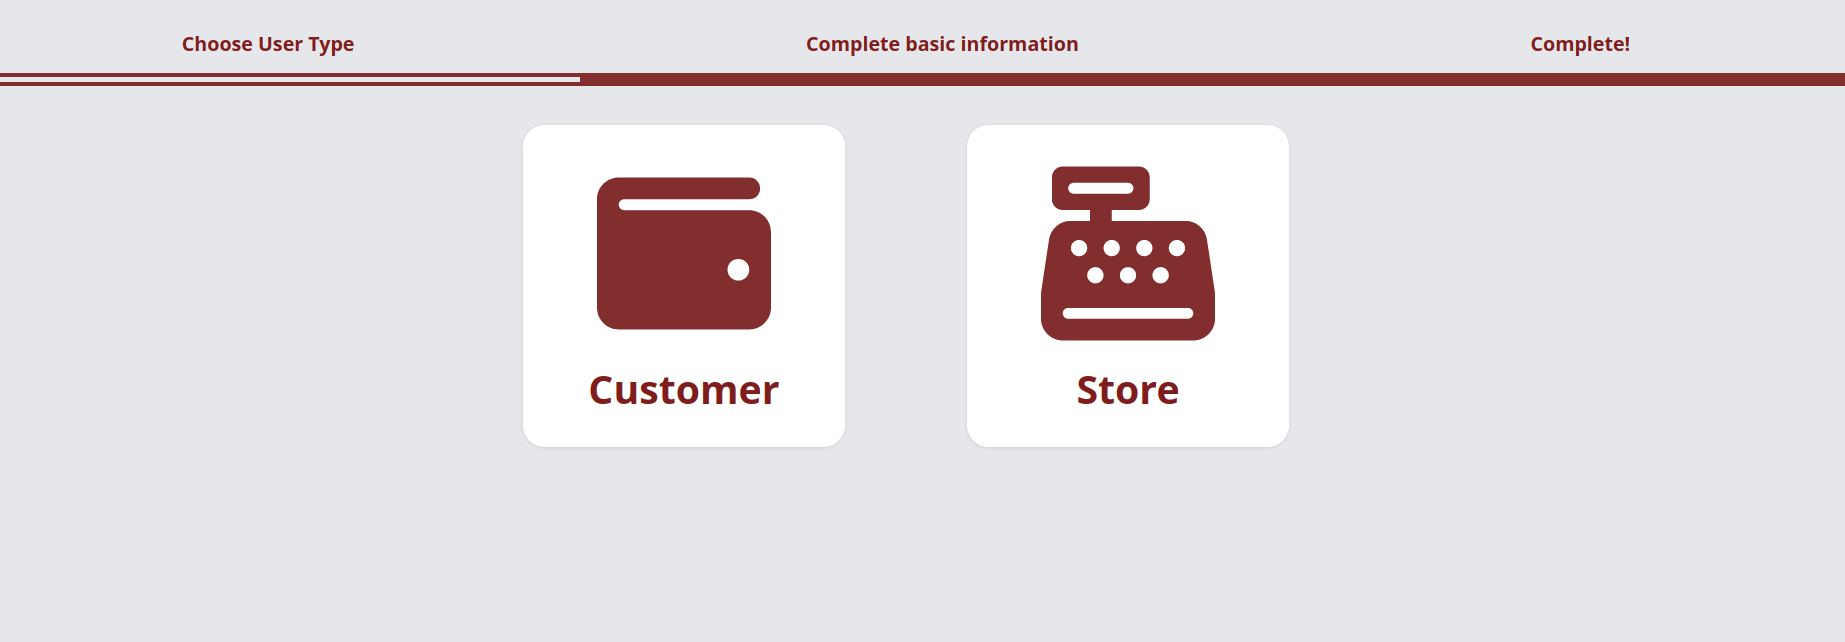
\includegraphics[width=40em]{gui-snapshot/user/register-customer-1.png}}
    \label{fig:enter-label}
\end{figure}
\begin{figure}[hp]
    \centerline{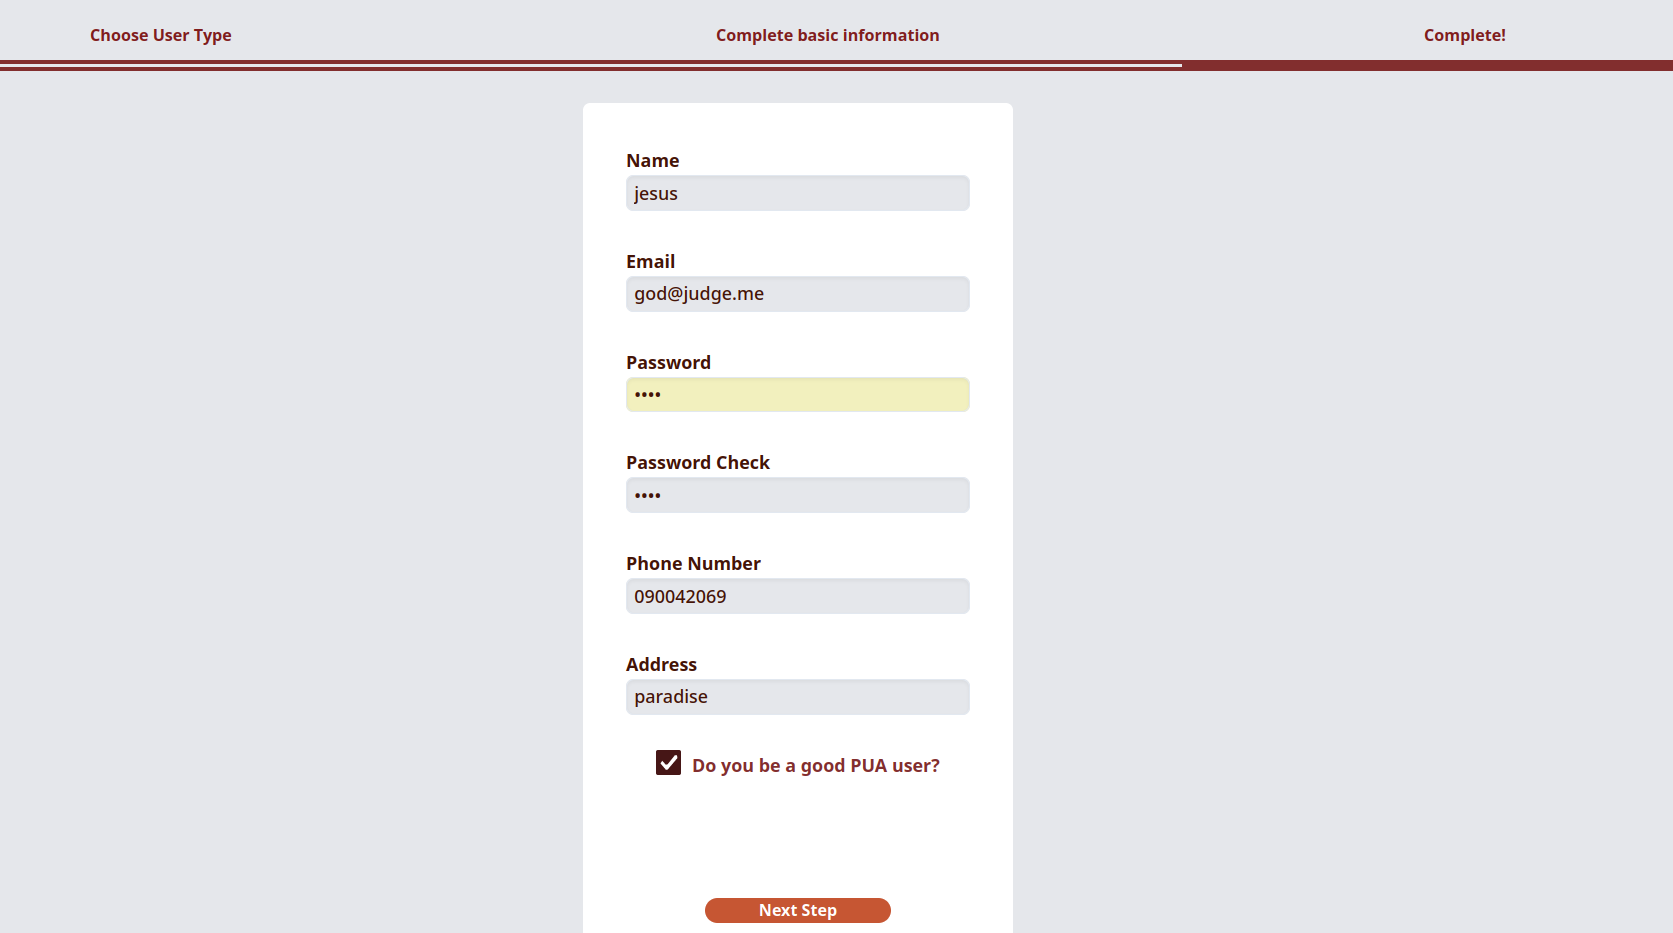
\includegraphics[width=40em]{gui-snapshot/user/register-customer-2.png}}
    \label{fig:enter-label}
\end{figure}
\newpage

\begin{figure}[hp]
    \centerline{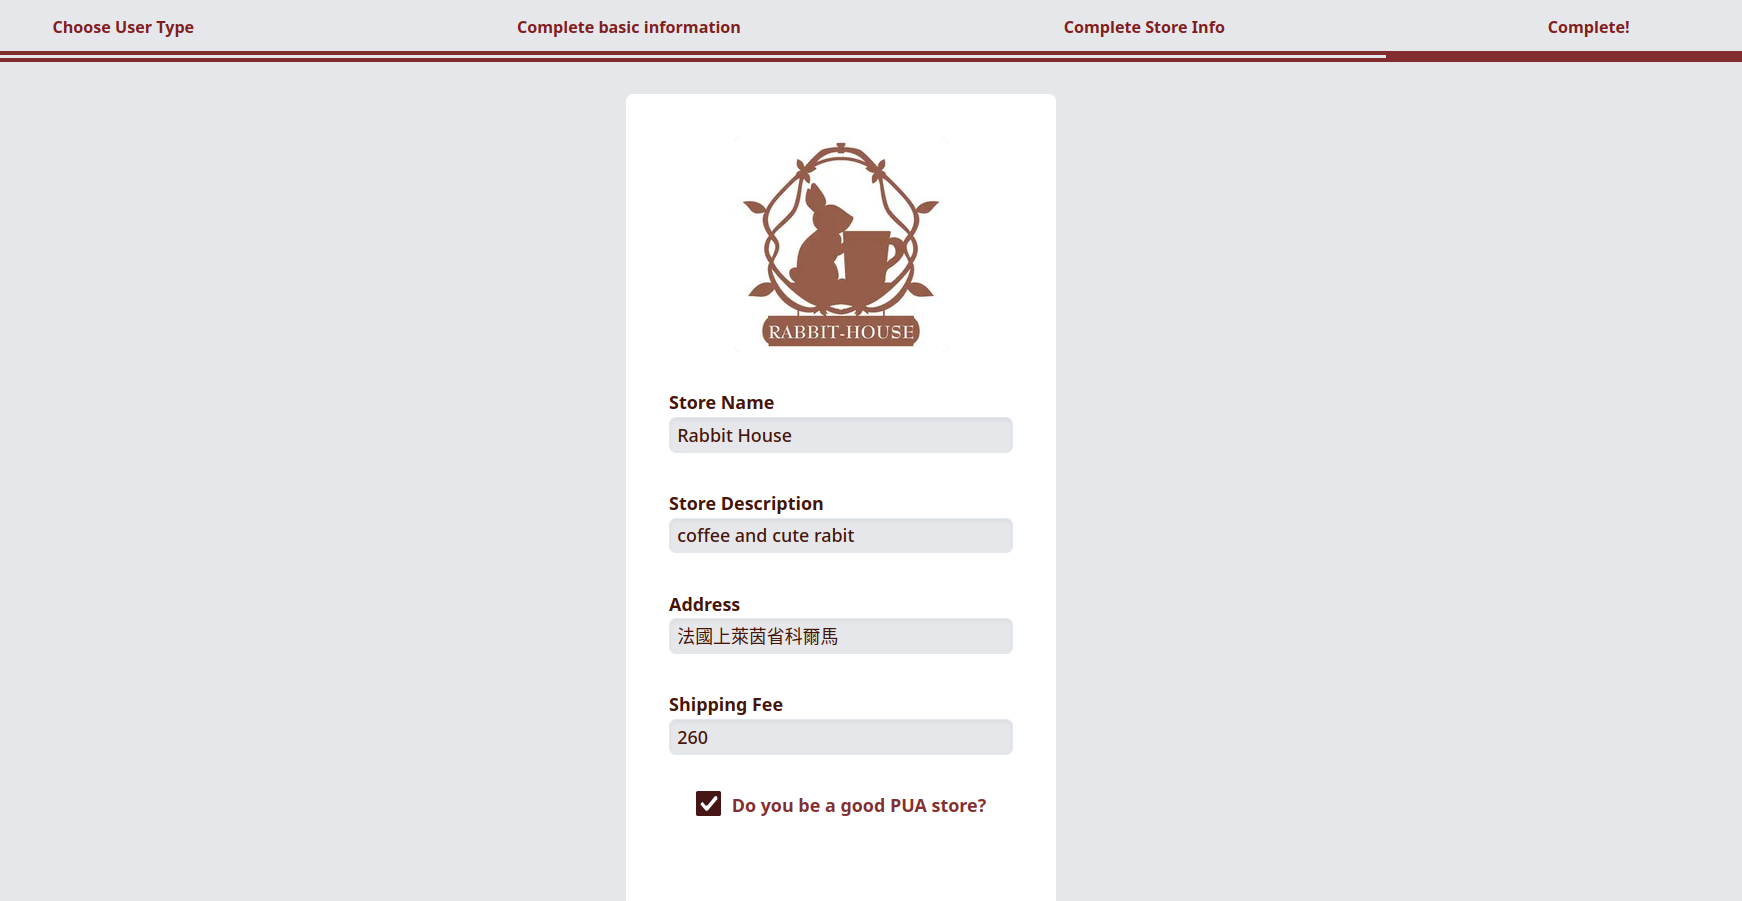
\includegraphics[width=40em]{gui-snapshot/user/register-seller.png}}
    \label{fig:enter-label}
\end{figure}
\begin{figure}[hp]
    \centerline{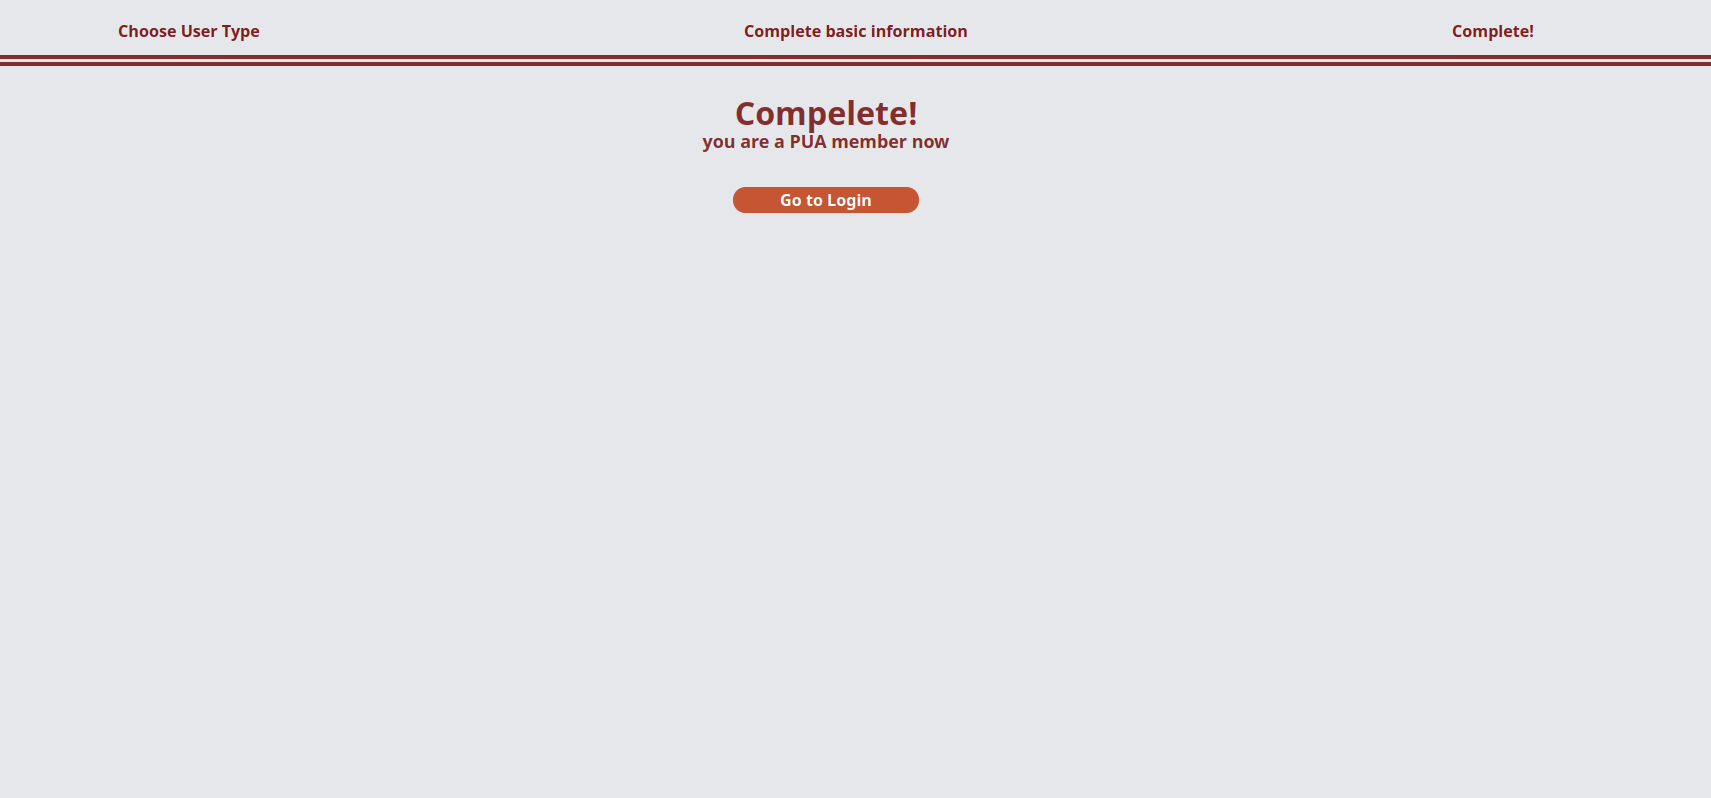
\includegraphics[width=40em]{gui-snapshot/user/register-customer-3.png}}
    \label{fig:enter-label}
\end{figure}
\newpage
\text{user can login (with PUA account or with TWP\cite{twp_project} account)}
\begin{figure}[hp]
    \centerline{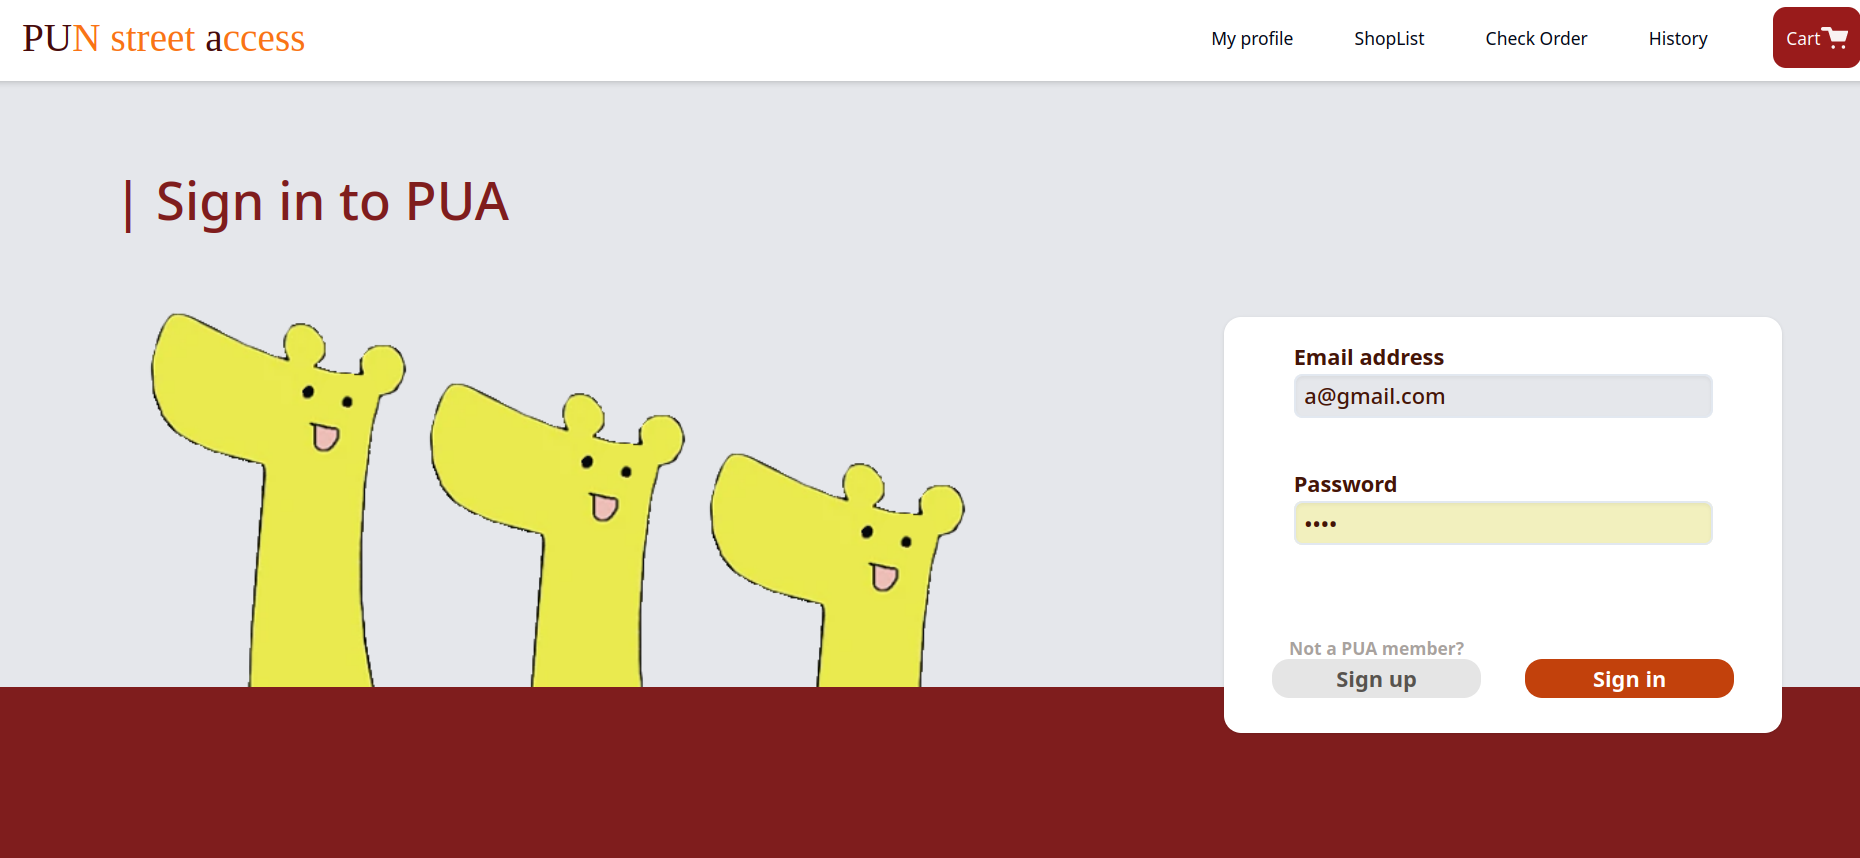
\includegraphics[width=40em]{gui-snapshot/user/login-page.png}}
    \label{fig:enter-label}
\end{figure}
\newpage

\subsubsection{customer}
\text{customer can browse shops}
\begin{figure}[hp]
    \centerline{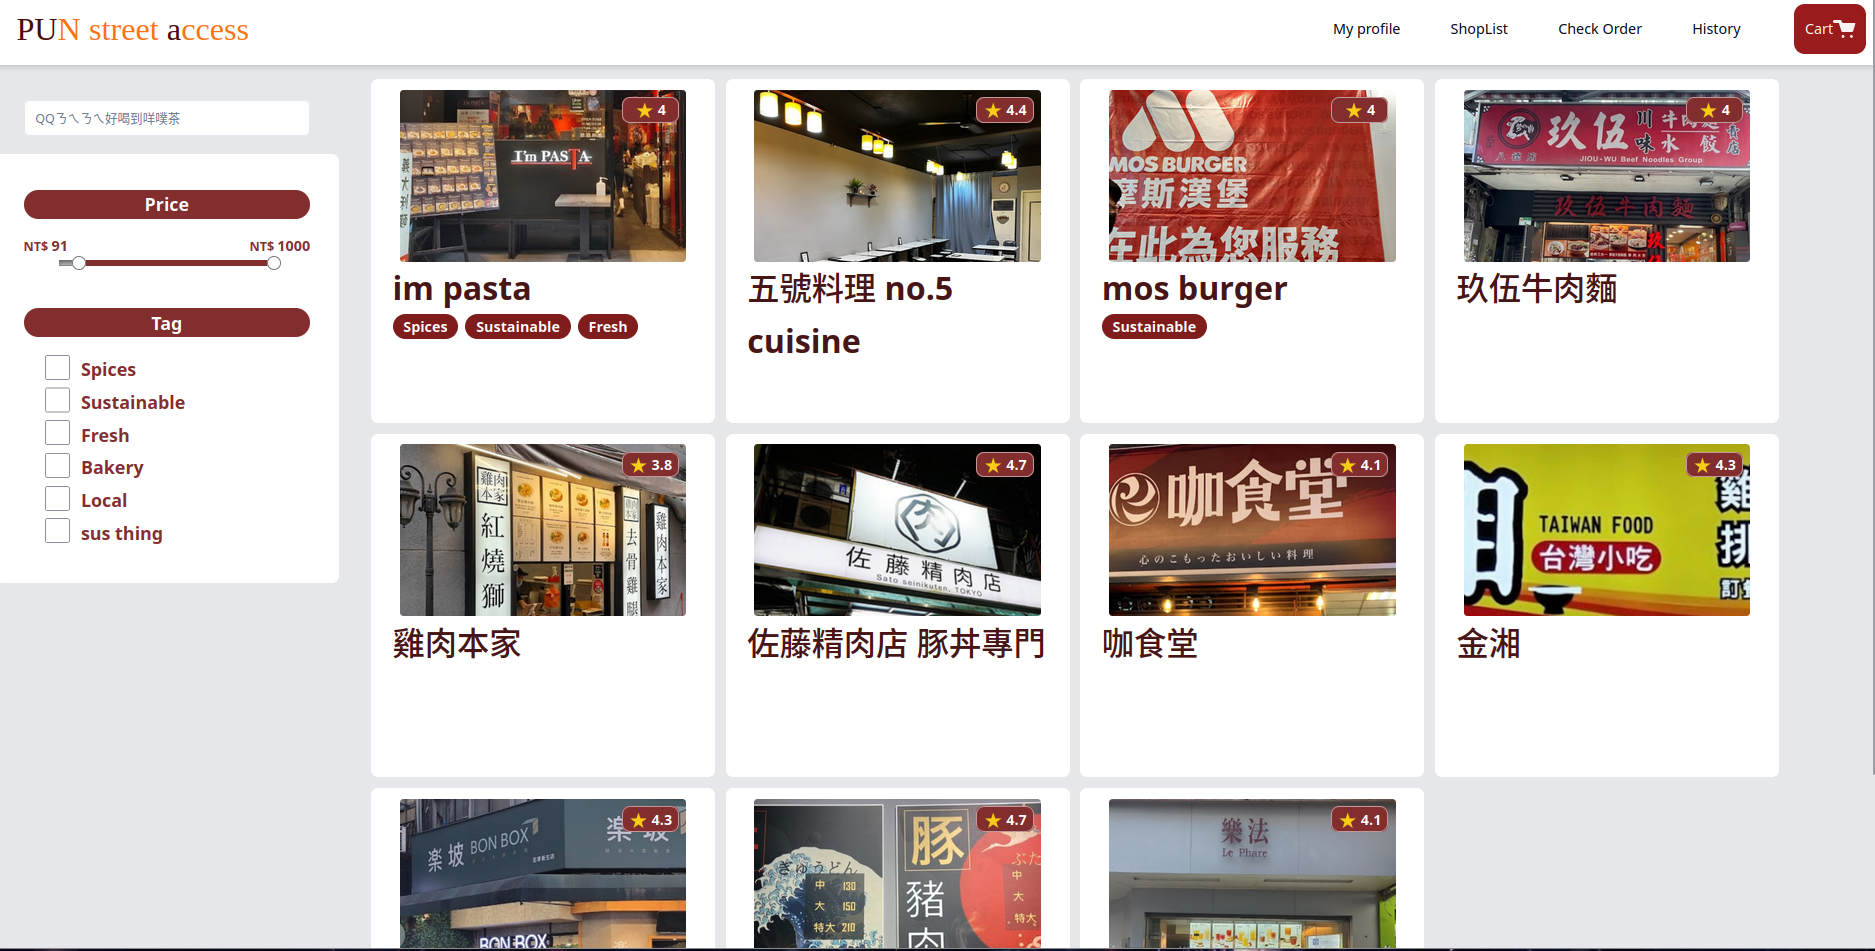
\includegraphics[width=40em]{gui-snapshot/customer/shoplist.png}}
    \label{fig:enter-label}
\end{figure}
\newline
\text{customer can search shops with price, tag or string}
\begin{figure}[hp]
    \centerline{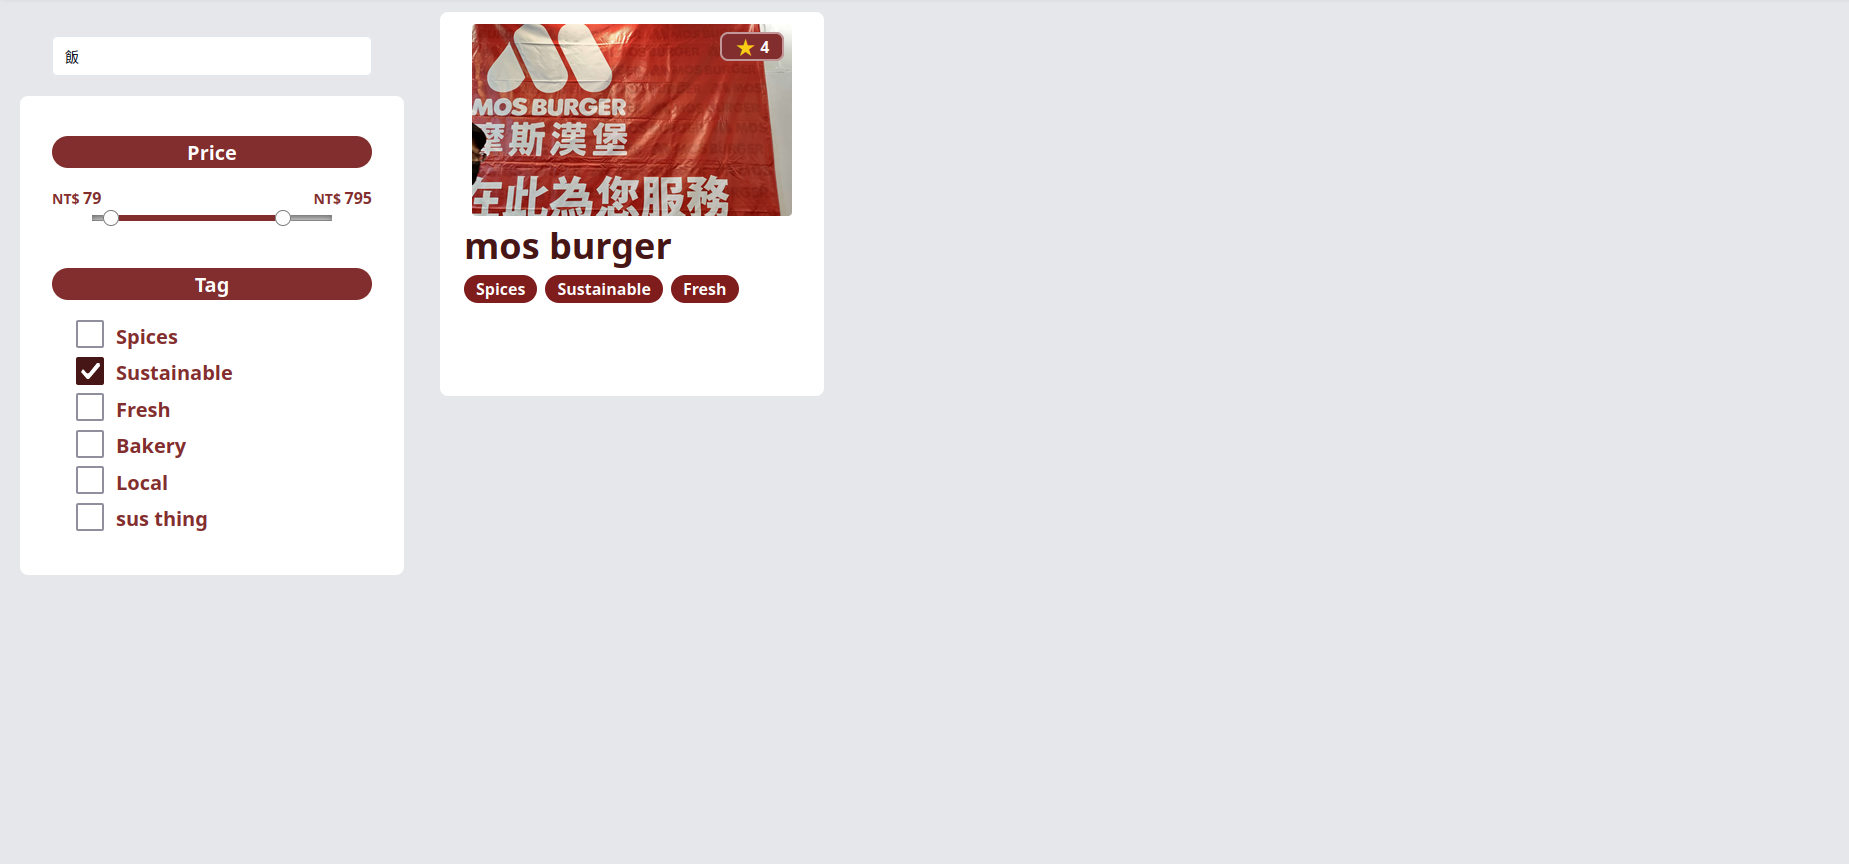
\includegraphics[width=40em]{gui-snapshot/customer/search.png}}
    \label{fig:enter-label}
\end{figure}
\newpage
\text{customer can browse products}
\begin{figure}[hp]
    \centerline{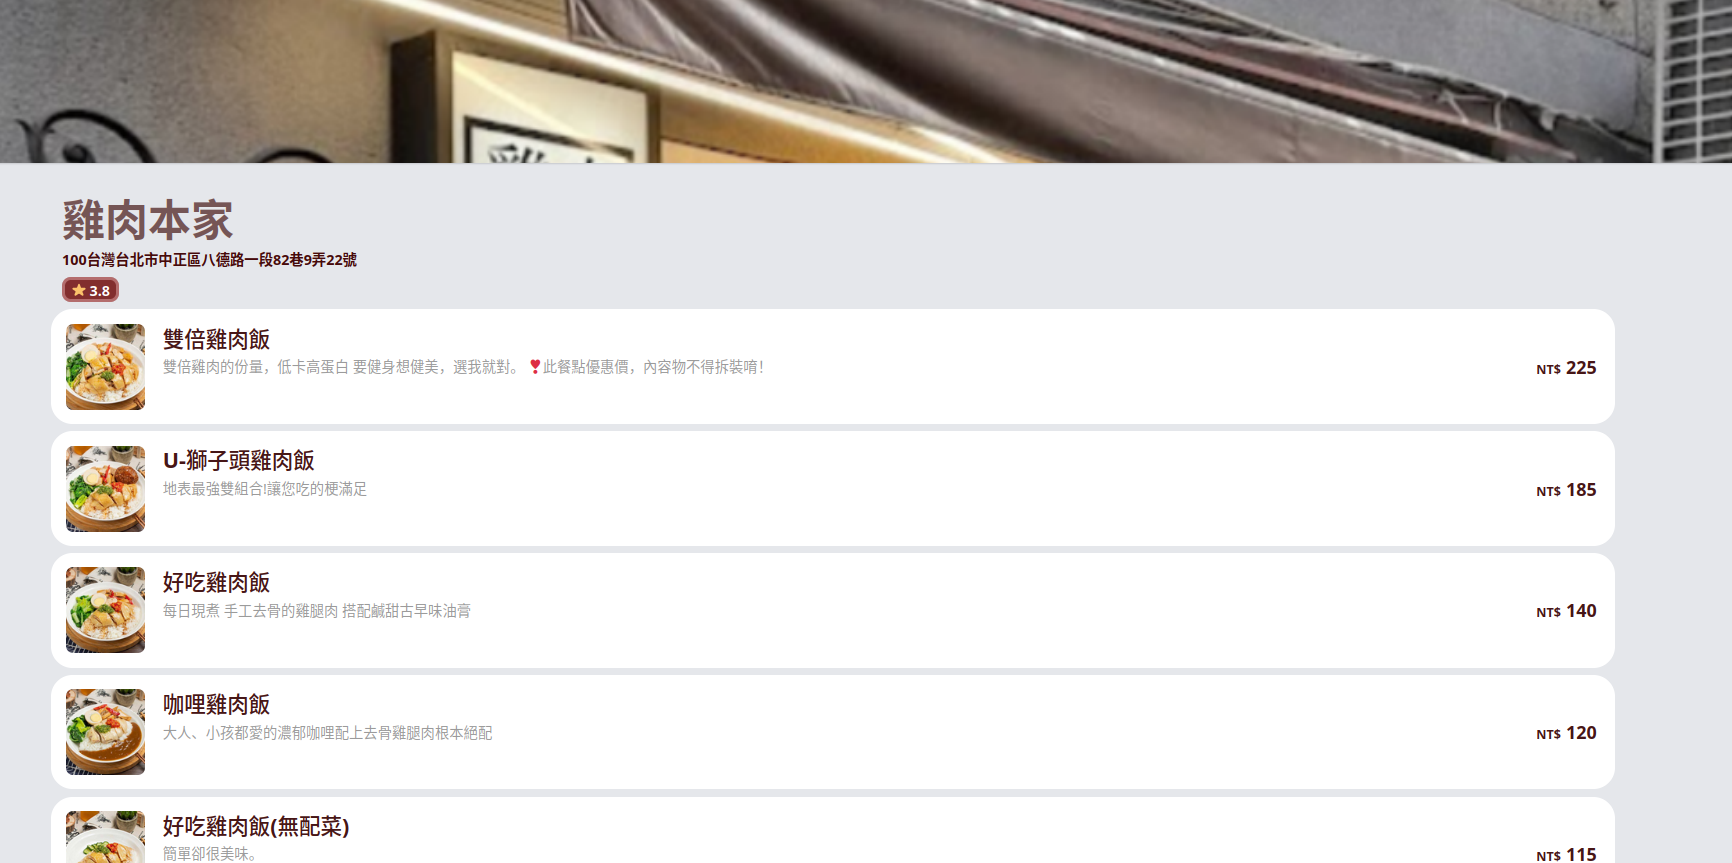
\includegraphics[width=40em]{gui-snapshot/customer/shop.png}}
    \label{fig:enter-label}
\end{figure}
\newline
\newpage
\text{customer can buy products}
\begin{figure}[hp]
    \centerline{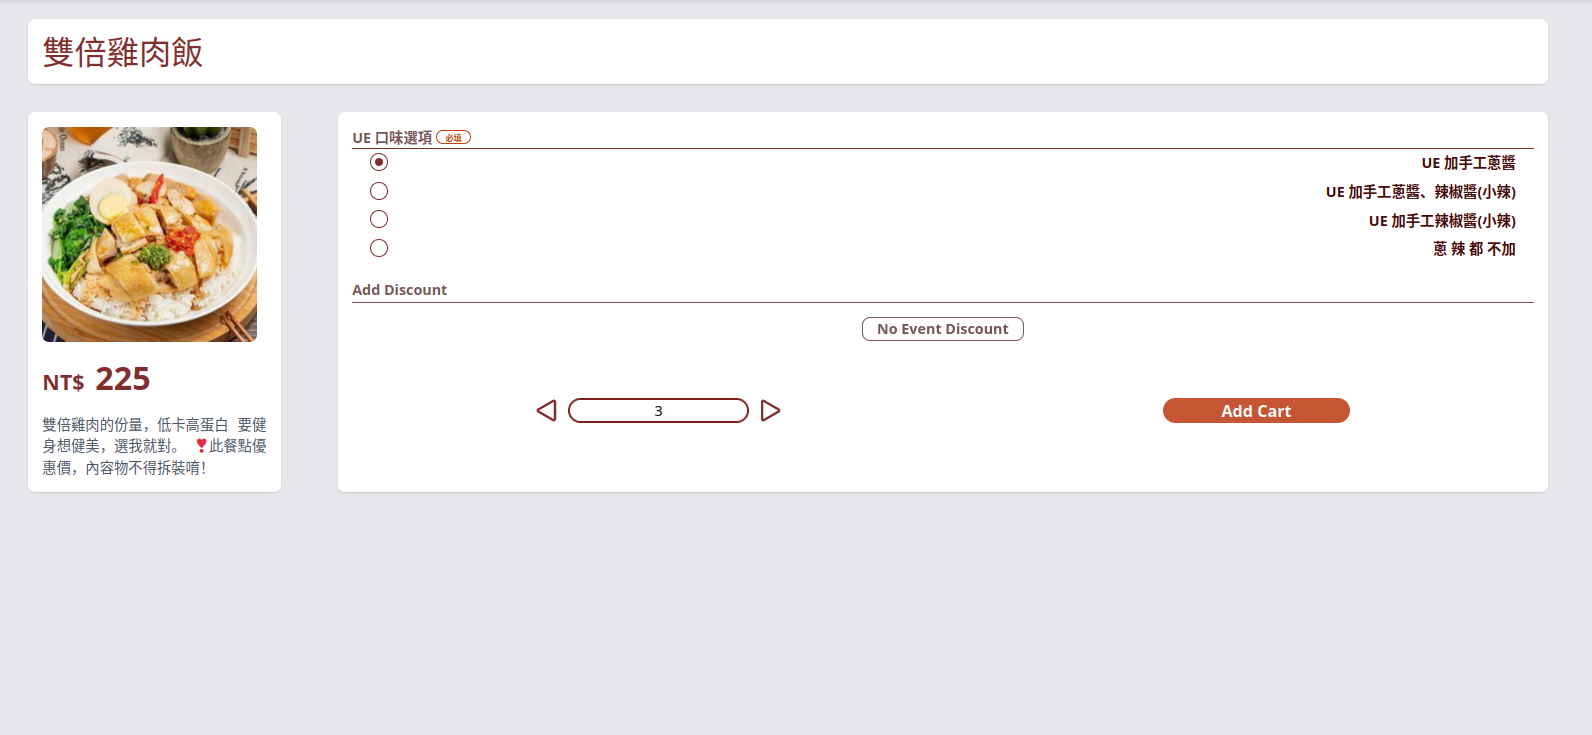
\includegraphics[width=40em]{gui-snapshot/customer/item.png}}
    \label{fig:enter-label}
\end{figure}
\newline
\text{customer can view cart (cart can apply discount)}
\begin{figure}[hp]
    \centerline{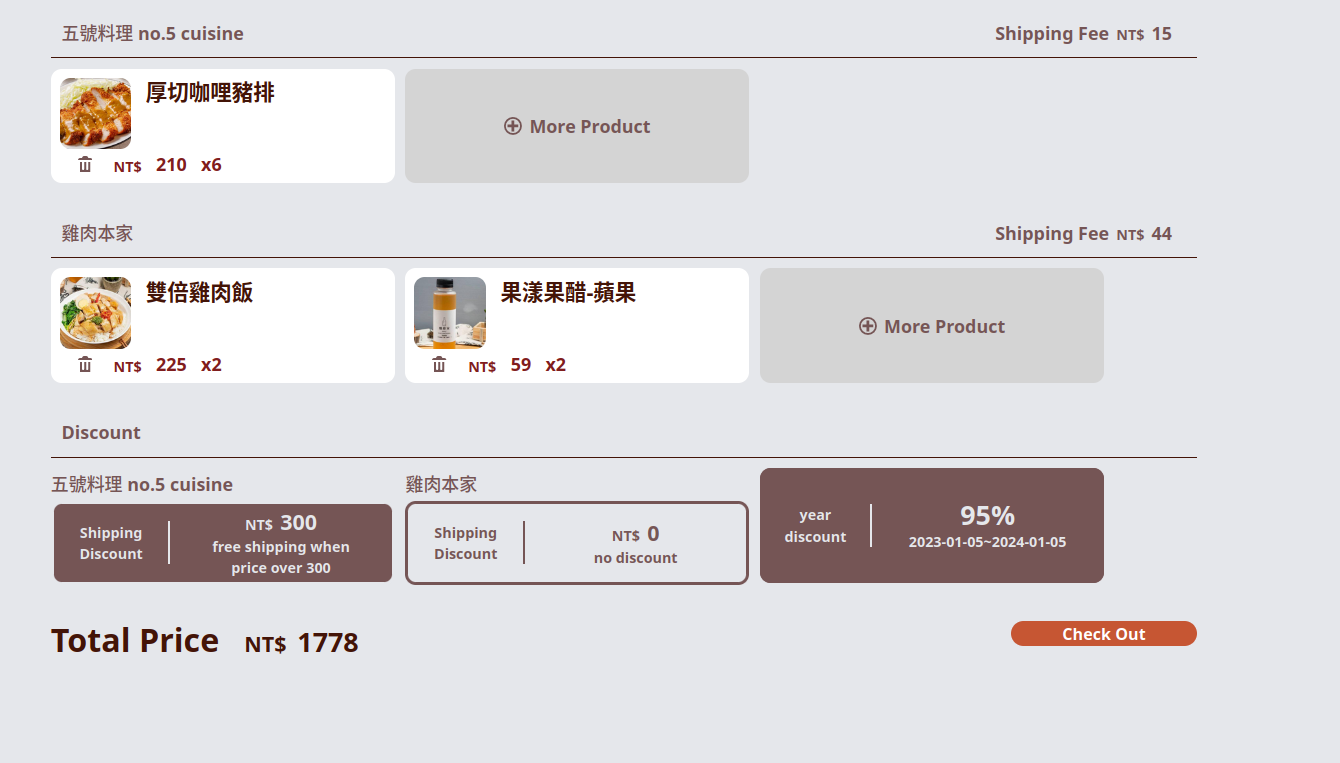
\includegraphics[width=40em]{gui-snapshot/customer/cart.png}}
    \label{fig:enter-label}
\end{figure}
\newpage
\text{customer can view order}
\begin{figure}[hp]
    \centerline{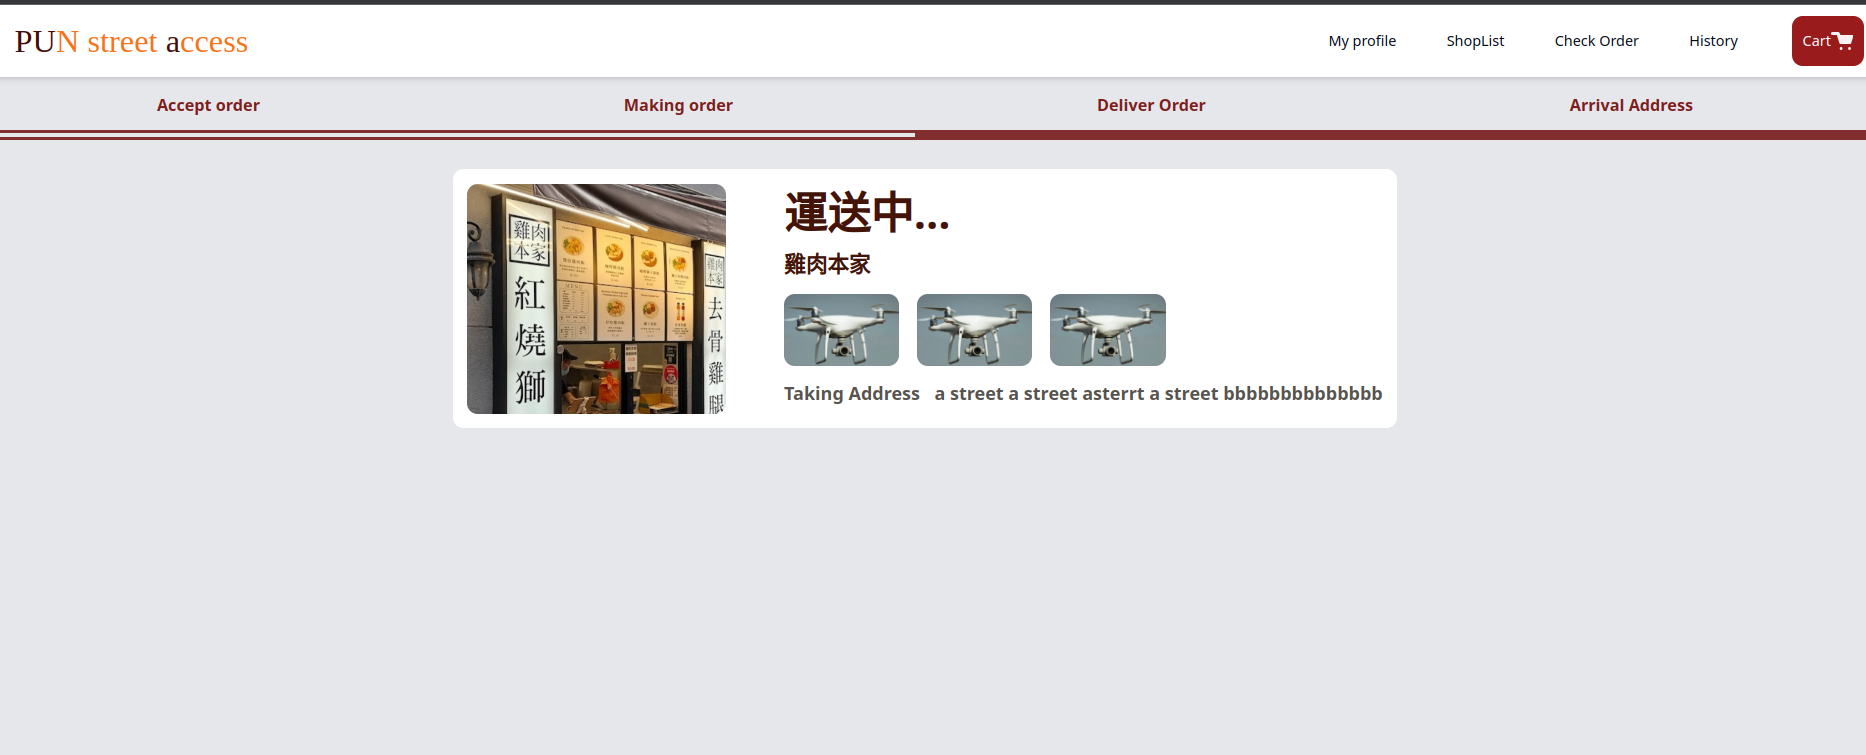
\includegraphics[width=40em]{gui-snapshot/customer/check-order.png}}
    \label{fig:enter-label}
\end{figure}
\newline
\text{customer can view history}
\begin{figure}[hp]
    \centerline{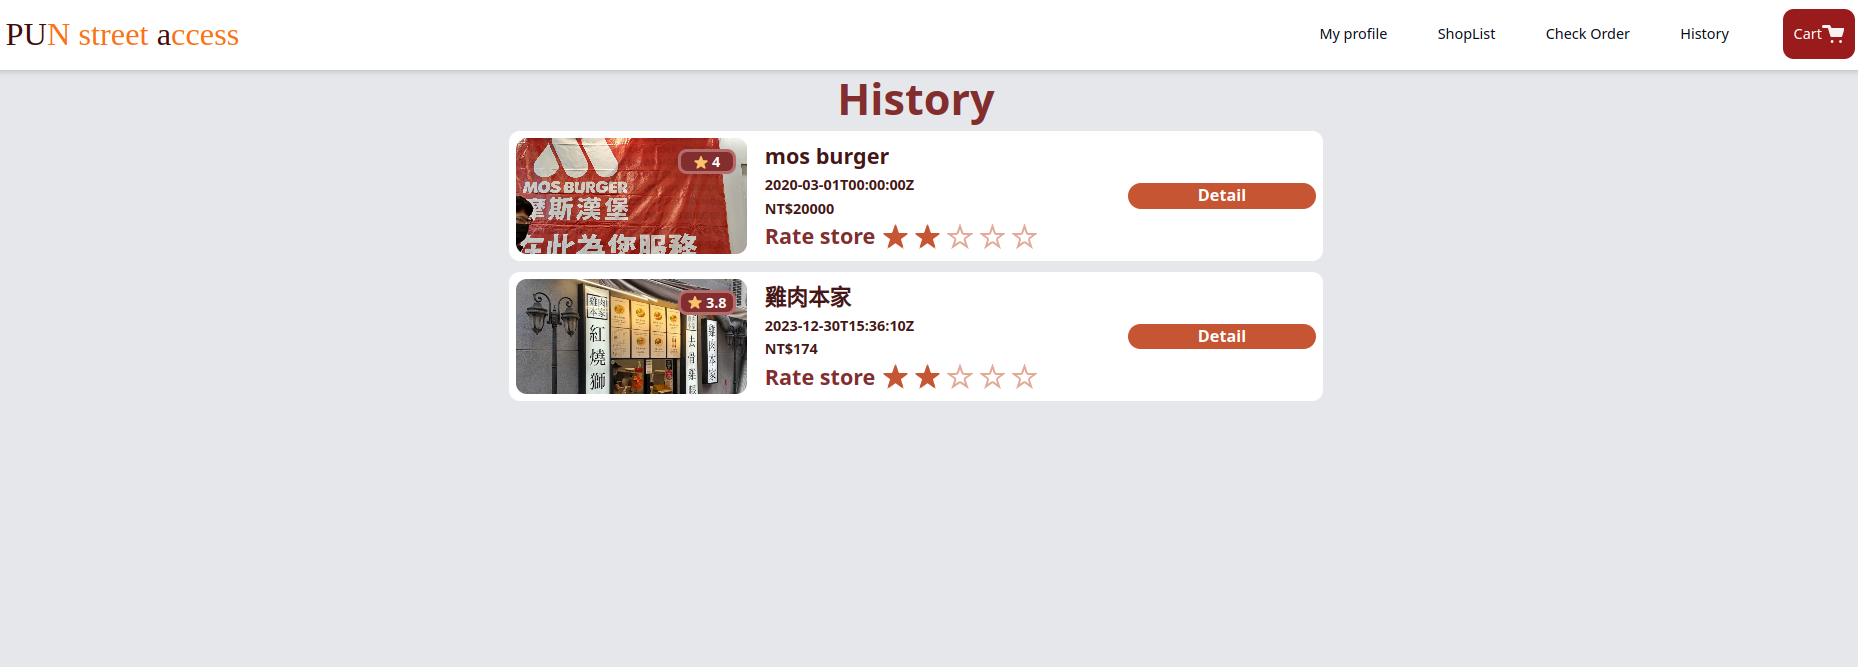
\includegraphics[width=40em]{gui-snapshot/customer/history.png}}
    \label{fig:enter-label}
\end{figure}
\newline
\newpage

\subsubsection{seller}
\text{seller can edit shop (edit tag)}
\begin{figure}[hp]
    \centerline{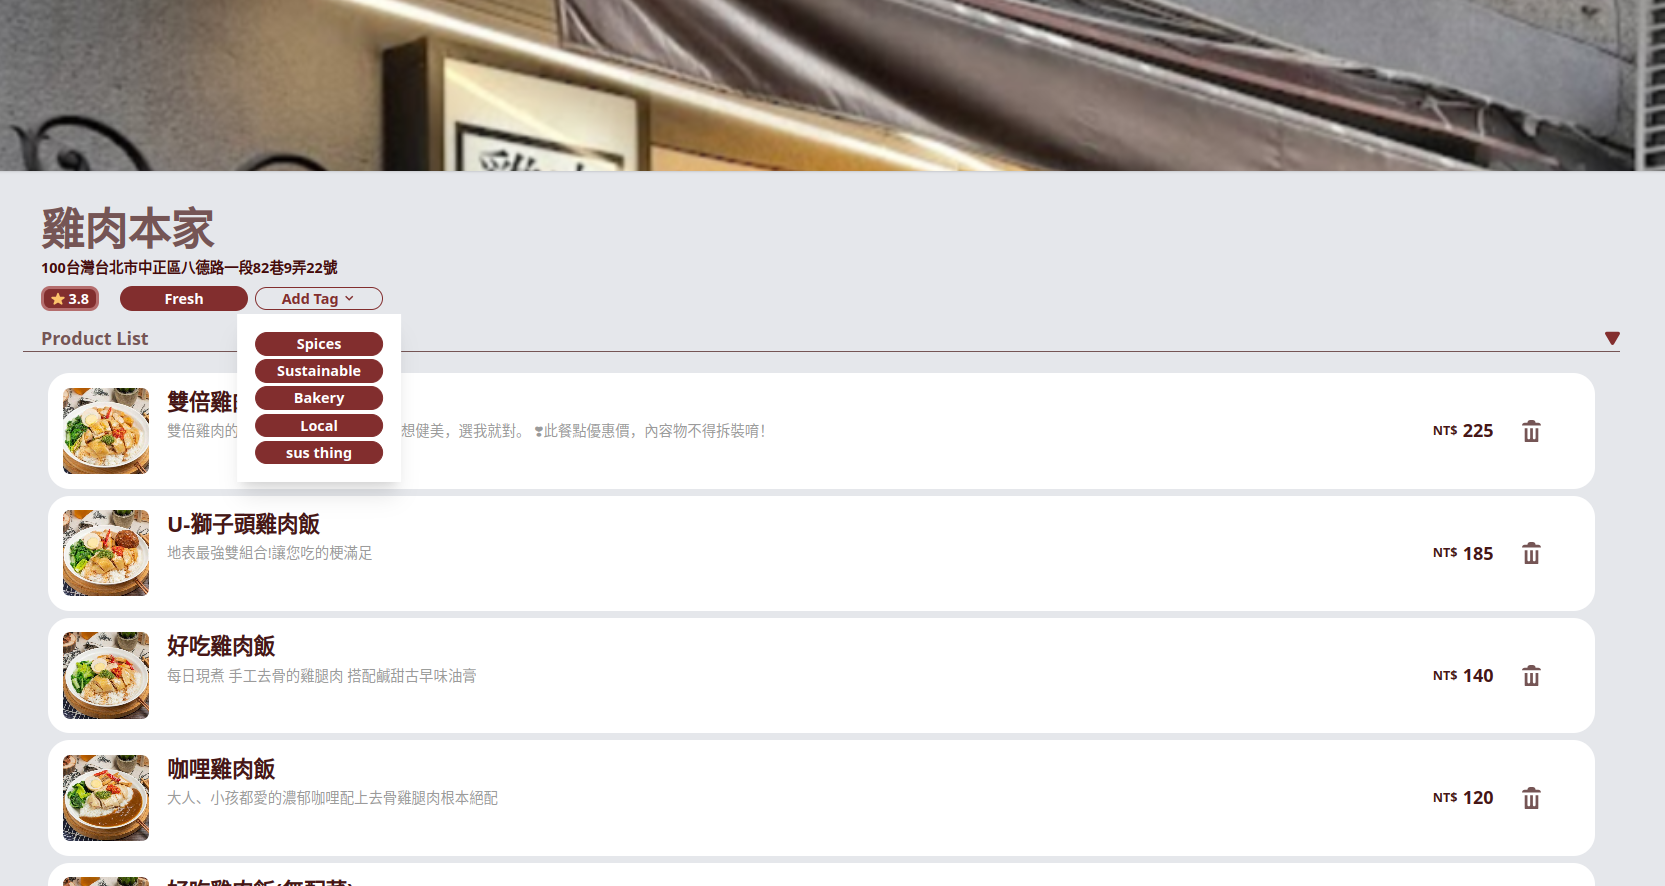
\includegraphics[width=40em]{gui-snapshot/seller/store-edit.png}}
    \label{fig:enter-label}
\end{figure}
\newline
\text{seller can edit (create) products}
\begin{figure}[hp]
    \centerline{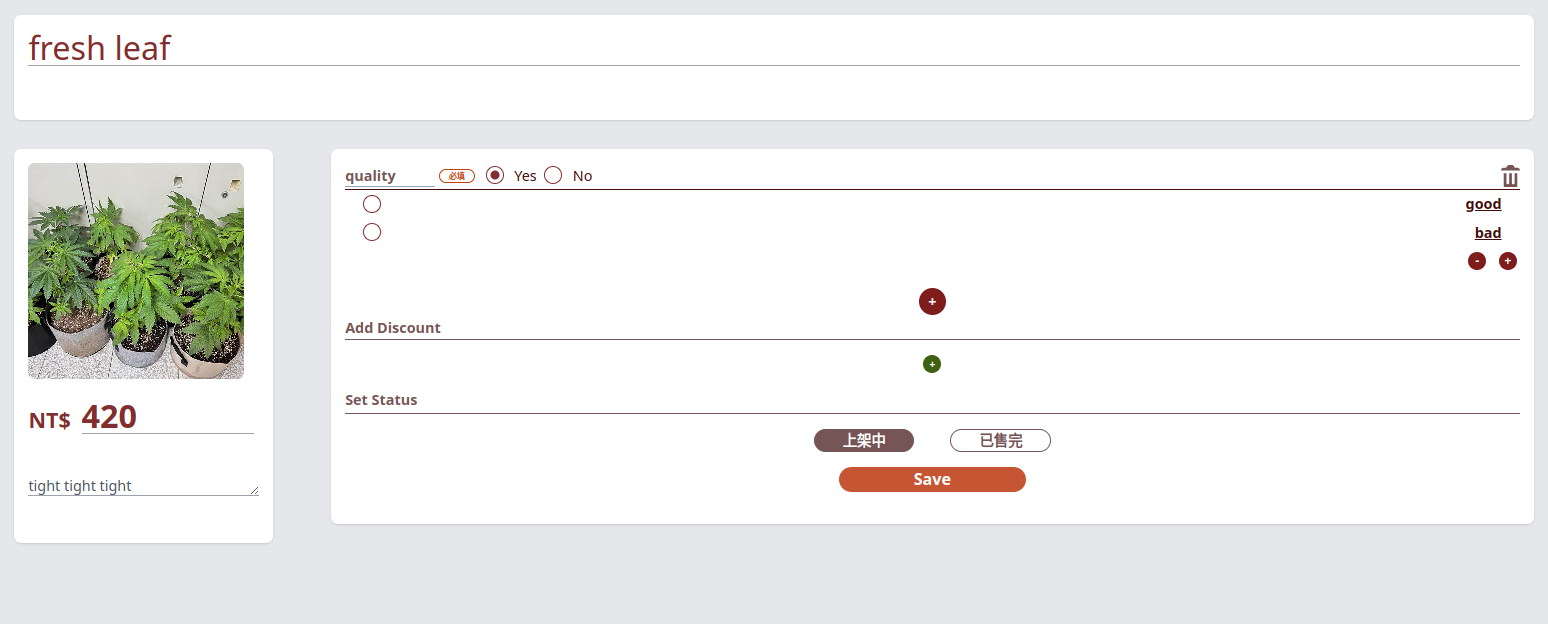
\includegraphics[width=40em]{gui-snapshot/seller/item.png}}
    \label{fig:enter-label}
\end{figure}
\newpage
\text{seller can edit (create) discounts}
\begin{figure}[hp]
    \centerline{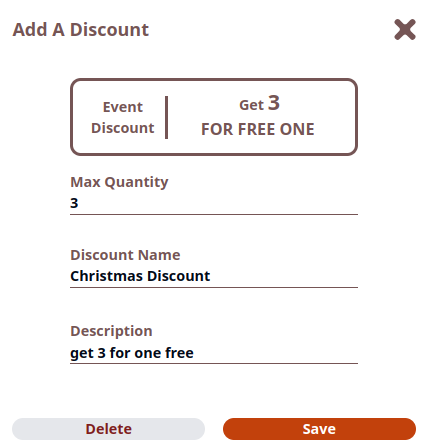
\includegraphics[width=20em]{gui-snapshot/seller/discount.png}}
    \label{fig:enter-label}
\end{figure}
\newline
\text{seller can view and update order}
\begin{figure}[hp]
    \centerline{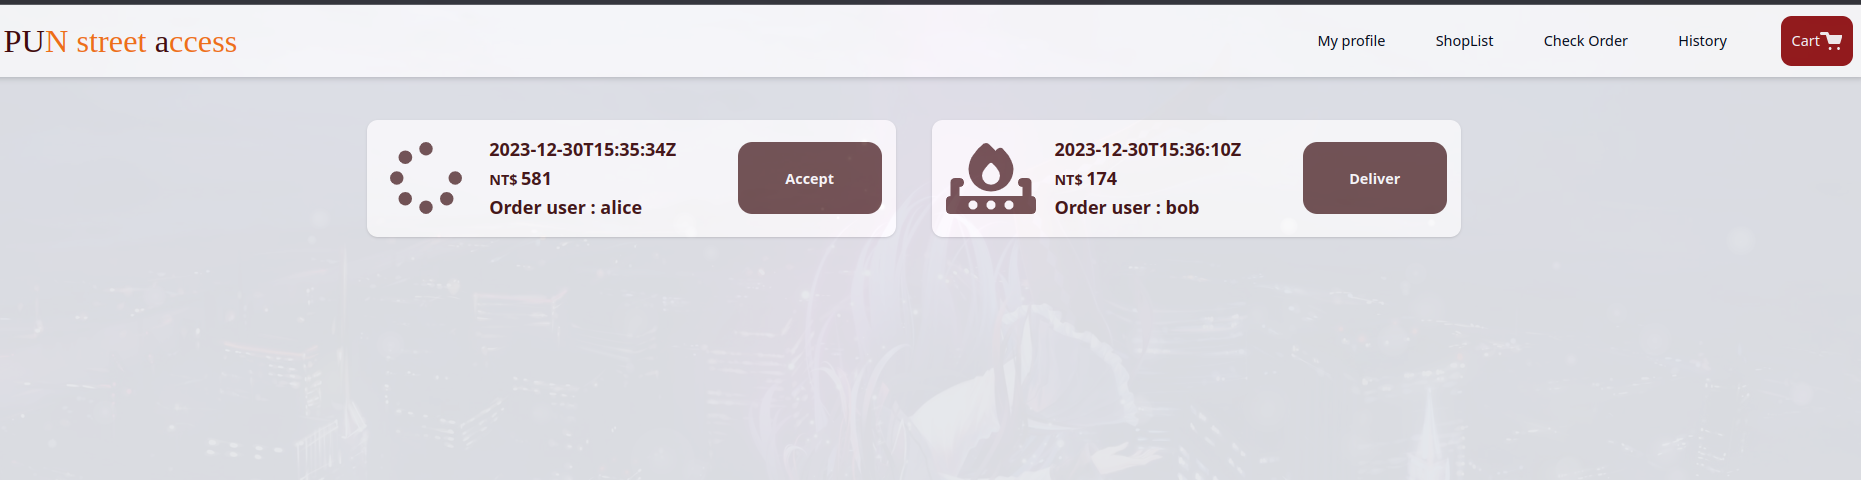
\includegraphics[width=40em]{gui-snapshot/seller/order-status.png}}
    \label{fig:enter-label}
\end{figure}
\newpage
\text{seller can get statistics of the shop}
\begin{figure}[hp]
    \centerline{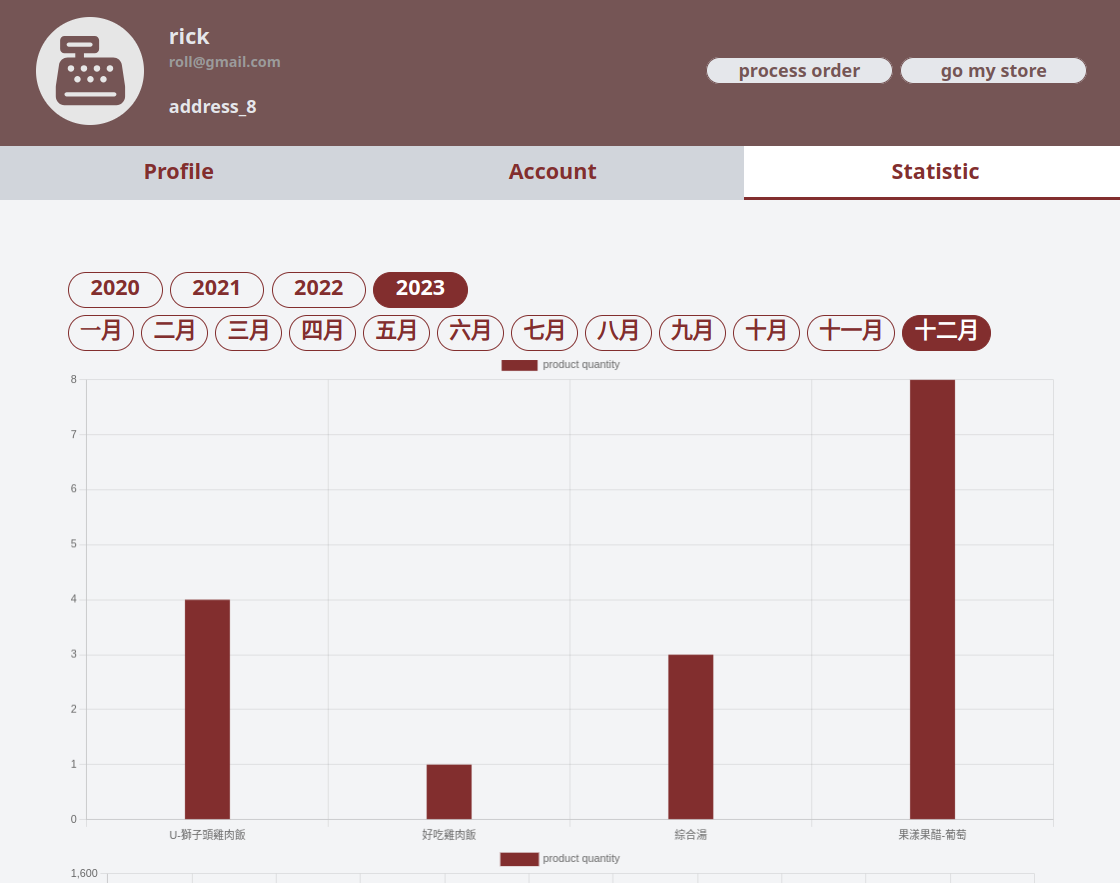
\includegraphics[width=30em]{gui-snapshot/seller/statistic.png}}
    \label{fig:enter-label}
\end{figure}
\begin{figure}[hp]
    \centerline{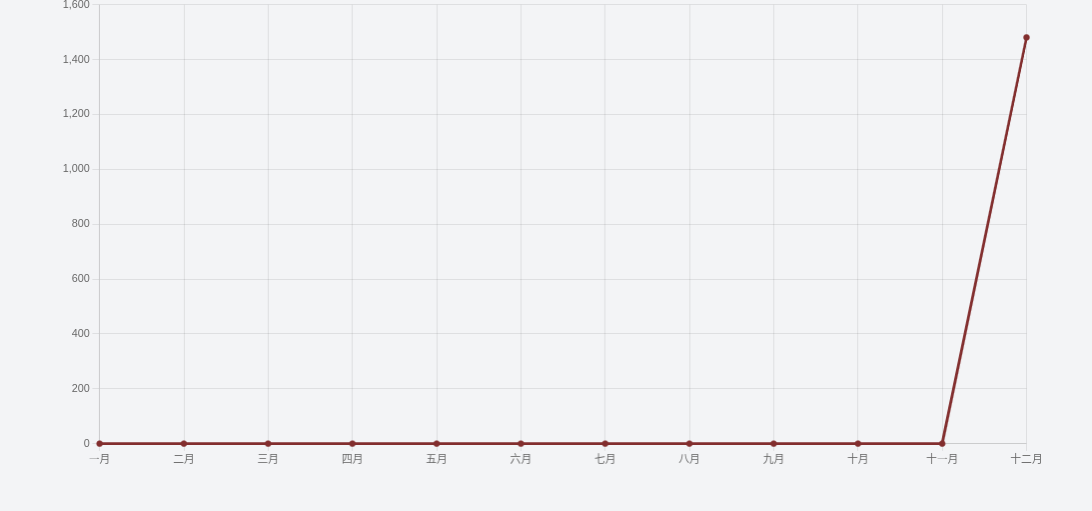
\includegraphics[width=30em]{gui-snapshot/seller/statistic-1.png}}
    \label{fig:enter-label}
\end{figure}
\newpage

\subsubsection{admin}

\text{admin can ban/unban users}
\begin{figure}[hp]
    \centerline{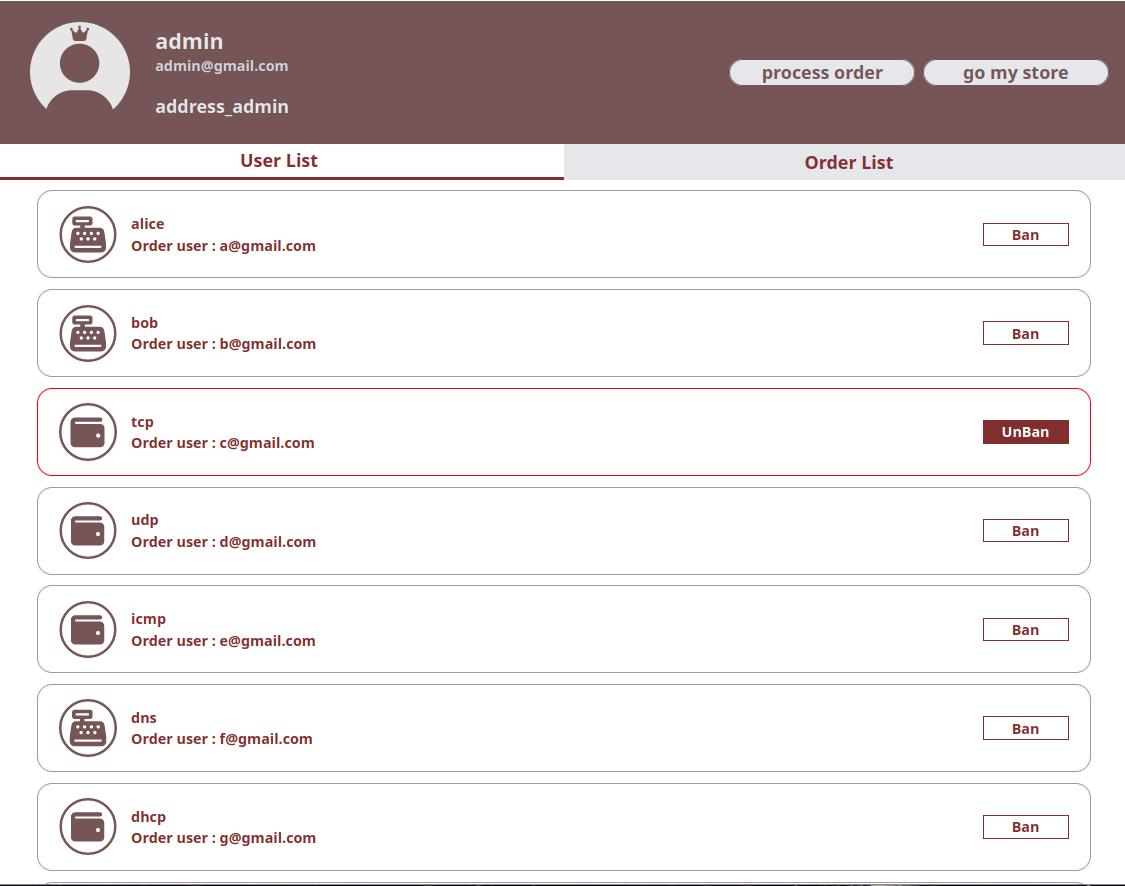
\includegraphics[width=40em]{gui-snapshot/admin/user.png}}
    \label{fig:enter-label}
\end{figure}
\newpage
\text{admin can view all orders}
\begin{figure}[hp]
    \centerline{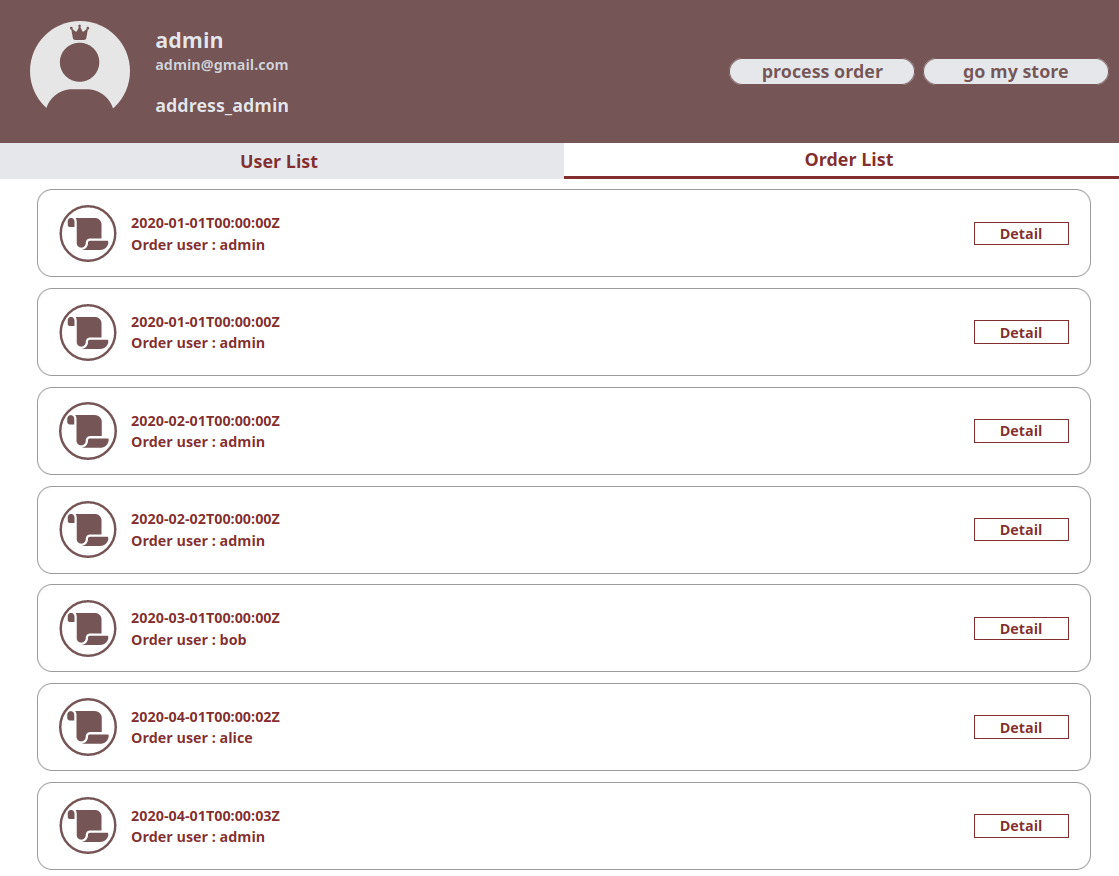
\includegraphics[width=40em]{gui-snapshot/admin/order.png}}
    \label{fig:enter-label}
\end{figure}

\newpage


\section{Suggestions on Database Turning}

\subsection{View}
    在取得商店或商品資料時,常常需要join許多不同的表格,若建立良好的view,可使得開發人員不需寫過於複雜的query,同時也增加資料可讀性。
\subsection{Index}
    在做搜尋功能時,其中有用到store中的category欄位,若能將category做為index,就可以避免線性搜尋所造成的效能損失。

\newpage

\section{Additional Queries and Views}

\subsection{First Query}

\text{Get shops by search string: use nest queries, aggregate functions, order by clause}
\begin{lstlisting}
SELECT
store_id,
name,
rate,
picture,
category_array
FROM (
    SELECT
        store_id,
        name,
        rate,
        picture, (
            SELECT
                jsonb_agg(
                    jsonb_build_object(
                        'category_id',
                        categories.category_id,
                        'category_name',
                        categories.name
                    )
                ) as categories_item
            FROM categories
                NATURAL JOIN (
                    SELECT labels.category_id
                    FROM labels
                    WHERE
                        labels.store_id = stores.store_id
                ) AS labels
        ) AS category_array, (
            SELECT COUNT(*) > 0
            FROM products
                LEFT JOIN stores as s ON products.store_id = stores.store_id
            WHERE
                products.store_id = stores.store_id
                AND(
                    products.name LIKE '%' || '飯' || '%'
                    OR stores.name LIKE '%' || '飯' || '%'
                    OR products.description LIKE '%' || '飯' || '%'
                )
        ) AS is_string_exits
    FROM stores
) as store
WHERE is_string_exits = true
ORDER BY store.rate DESC
\end{lstlisting}

\newpage
\text{query result}
\begin{figure}[hp]
    \centerline{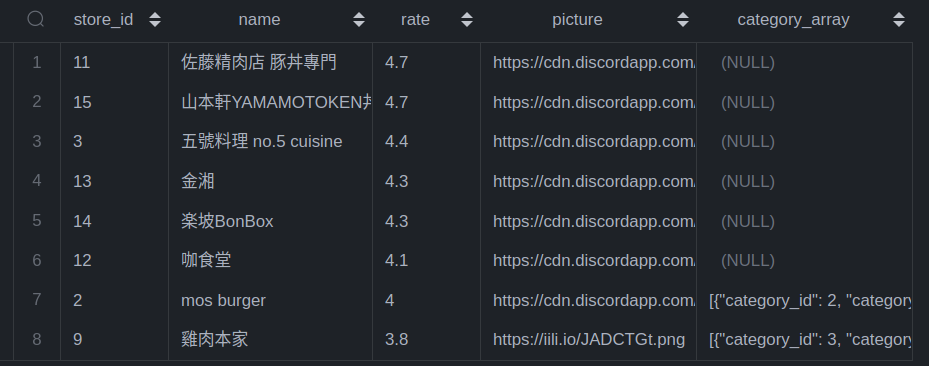
\includegraphics[width=40em]{result/result-1.png}}
    \label{fig:enter-label}
\end{figure}
\newline
\newpage

\subsection{Second Query}
\text{Get products selling statistics by date: use group by clause}
\begin{lstlisting}
SELECT
    carts.product_id,
    products.name,
    SUM(carts.product_quantity)
FROM carts
    LEFT JOIN products ON carts.product_id = products.product_id
    LEFT JOIN orders ON carts.store_id = orders.store_id AND carts.cart_id = orders.cart_id AND carts.customer_id = orders.user_id
WHERE
    orders.store_id = 1
    AND orders.status >= 6
    AND EXTRACT(
        year
        FROM
            order_date
    ) = 2020
    AND EXTRACT(
        month
        FROM order_date
    ) = 1
GROUP BY
    carts.product_id,
    products.name
\end{lstlisting}
\text{query result}
\begin{figure}[hp]
    \centerline{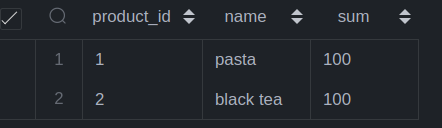
\includegraphics[width=30em]{result/result-2.png}}
    \label{fig:enter-label}
\end{figure}

\newpage

\subsection{Third Query}
\text{Get all Product's information: use nest query, order by clause}
\begin{lstlisting}
SELECT
    product_id,
    store_id,
    name,
    description,
    picture,
    stock,
    price,
    status, (
        SELECT
            coalesce(
                jsonb_agg(
                    jsonb_build_object(
                        'discount_max_quantity',
                        max_quantity,
                        'product_id',
                        product_id,
                        'discount_name',
                        name,
                        'discount_description',
                        description,
                        'discount_id',
                        discount_id,
                        'status',
                        status
                    )
                ),
                '[]'
            ) AS event_discount
        FROM discounts
            NATURAL JOIN (
                SELECT
                    event_discount.discount_id,
                    event_discount.max_quantity,
                    event_discount.product_id
                FROM event_discount
                WHERE
                    event_discount.product_id = products.product_id
            ) AS discountInfo
    ) AS event_discount_array, (
        SELECT
            coalesce(
                jsonb_agg(
                    jsonb_build_object(
                        'product_id',
                        product_id,
                        'label_name',
                        label_name,
                        'required',
                        required,
                        'item_array', (
                            SELECT (
                                    jsonb_agg(
                                        jsonb_build_object('name', label_item.item_name)
                                    )
                                ) AS item_array
                            FROM label_item
                            WHERE
                                label_item.label_name = product_label.label_name
                                AND label_item.product_id = product_label.product_id
                        )
                    )
                ),
                '[]'
            ) AS product_label_array
        FROM product_label
        WHERE
            product_label.product_id = products.product_id
    )
FROM products
WHERE store_id = 1 AND status != 0
ORDER BY product_id;
\end{lstlisting}
\text{query result}
\begin{figure}[hp]
    \centerline{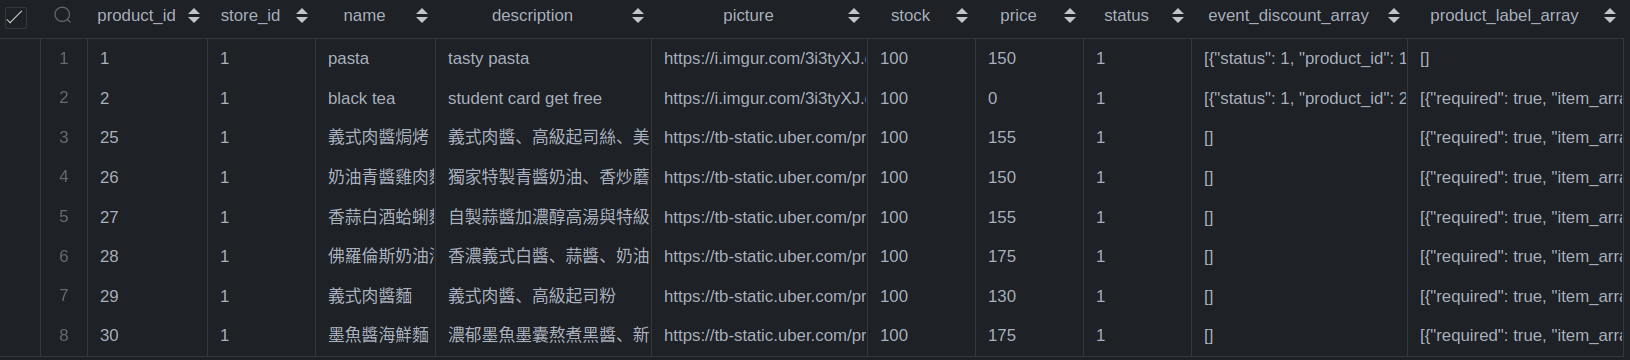
\includegraphics[width=40em]{result/result-3.png}}
    \label{fig:enter-label}
\end{figure}

\newpage

\section{Conclusions and Future Work}
\subsection{Conclusions}
\begin{itemize}
    \item[郭丞軒] 
    這次專案的開發涉及許多領域,從團隊管理、資料庫設計、到文件撰寫及前後端架構等,很多東西都是我第一次接觸。因此,常常在開發過程中搞砸許多事情,造成開發上的困難以及不斷的重構。但也很幸運地受到組員們及組外顧問的幫助,得以讓這次的專案順利進行,也讓我從中得到許多寶貴的經驗。
    \item[王熯竑] 
    這次的專案開發是我第一次接觸前.後.後.資料庫端網頁程式設計,也是我第一次接近管理專案,導致需要看很多code review,進而使用github action與npm lint幫助我管理專案,在中途有很多PR都因爲我身兼拆除炸彈的使命與另外一個專案管理的事情還有與Dr.Smell對抗的學分競爭,導致拖延很多個禮拜才進行code review,幸好有生產力爆發的組員才得以順利完成專案。在前後端溝通的問題或是組內資訊流通的問題,我使用了每個禮拜發佈一個週報來解決,他可以順便當成一個Todo-List,雖然最後證實他沒有很大幫助,但是他取代了每次都不知道要開甚麼的會議,節省了時間。
    
    在資料庫設計的部分有很多綱要的決策常被忘記,導致又花了很多時間得到一摸一樣的結論,需要hyjl(會議記錄,出自本地顧問)來解決這個問題。

    前端的部分使用的svelte是非常有趣的框架,他擁有魔法的語法,加速我們的開發進度,他的缺點大概就是網路上的資料常常會過期,需要另外解決。Tailwind也是另外一個非常好框架,有邏輯的解決了css問題,網頁跑版的問題才可以縮到很小,但是礙於時間問題沒有處理RWD。
    \item[陸艿寰] 
    透過這次資料庫專案,我學到了資料庫除了只有儲存資料,還有它背後儲存資料時所需的複雜邏輯與規則、及使其運行所需的軟/硬體。在專案中我主要接觸到了UI製作,並學習到了製作及實現他人設計的困難之處與其解決方法。

    專案製作中還有許多其他關鍵的技術。如設計資料庫架構、實現資料庫邏輯、銜接資料庫與UI功能...等。這些技術的製作過程讓我學習到各功能製作者互相溝通是非常重要的事情,必須充分交流、協調才能避免製作遇上瓶頸。

    最後各階段報告時老師的指點也讓我受益良多,以淺顯易懂的話語指出設計或實作的瑕疵/不足,讓我們有機會回去修改,拿出更好的成果。
    \item[陳姿安] 
    這次專案幾乎所有事情都是初次體驗。

    在專案負責後端部份,初次與golang相處一段時間後發現寫起來覺得蠻舒適的,且我們採用的框架將後端切得很乾淨寫起來非常順手。
    
    此次也獲得了一些文件撰寫的經驗、也經歷的重構文件的經驗,相信下次設計api的時候會更順利。
    透過這個專案我也獲得了設計網頁界面的經驗,從來沒想過自己會有設計網頁的一天,雖然實做不是由自己完成,但是看到自己設計的UI被慢慢實踐出來很開心,每天看到都想修改但這對負責實做的人並不是很道德,所以我放棄了這樣的想法。

    也因為負責了後端所以有機會寫到不少sql,起初以為sql只是insert select update一些簡單的操作,後來上課後才發現原來sql可以寫的相當複雜,且好的魔法sql可以將網頁的效率提高,sql想寫多長就有多長。
    親切的組員讓我當慣老闆,我非常的開心,希望以後還有機會當慣老闆。
    \item[劉承翰]
    資料庫這門課讓連後端都沒碰過的我第一次知道後端的概念與做法,在實作的過程中還發現有從計算機網路學到的概念可以結合使用,發現還挺有趣的。雖然整體沒辦法貢獻太多(sorry),開PR還常常被拒絕,但看其他coding實力強的人寫code也學到蠻多東西的。這次花最久的時間應該就是看code了吧,每次有新的PR就會嘗試理解它的原理,也趁機會學習一下架構與別人的coding style:D。
   \item[歐佳昀]
    經過資料庫系統的專案後,我對於資料庫系統的應用有了更深一層的認知,並且也有實際的感覺,原來他不僅僅是作為一門學科,更是資工系學生在開發一個電商專案時,實際會用到的知識。
    而在專案中,除了資料庫的基礎知識運用外,我也獲得相當多的經驗,像是前端的開發、 ui 的設計、與人交流、溝通的技巧等等,或者是分析一個網站的需求,諸如使用的情境,細節等,更重要的是去實際體會了投入心血的感覺,並且在樂在其中,這才是最重要的。

    我堅信,一份作業需要帶給學生的,不僅僅是對知識運用的掌握度,更是需要帶給學生新的體驗與認識,而團體的作業更是能體會到不同思維間的碰撞。而我在最後深刻去了解老師說的話,為何這份作業,卻希望我們能放在自己未來的履歷上 ? 更是因為這是我們從頭開始去作出的專案,因此才具有理解和掌握,與認知和成就感。 

    這份專案的完成,而掌握到的知識,不管是討論各項系統與api,或者是邏輯性的去提出自己的需求,甚至是自我學習的能力,都是我在這份專案有所學、有所悟的地方,也希望在未來可以充分運用這些經驗,來補足自己的能力。
    \item[組外顧問]
    我的專業在這個組別得到比原本組別更多的尊重,10 / 10 推薦擔任顧問 
\end{itemize}

\subsection{Future Work}
PUA 目前已經是個非常完善的系統,未來的目標是將其統推廣到全校以及北科周圍的店家,並引入無人機作為外送載體,不只節省人力成本,也使得狹小的美食街不再充滿汽、機車,帶給商家及學生更美好的環境。

我們也計畫在之後與『太白粉專賣店 too white powder (TWP)』合作,讓商家可以透過PUA向TWP訂購原物料,使供應鏈管理更為便利。

\newpage

\section{References}
\printbibliography[heading=none]
\newpage

\section{Appendix}
Demo video link \href{https://www.youtube.com/playlist?list=PLBGxrBkKAa3qo2uLVUKfLOQeE1iUDgnIc}{link} 

The link to the system deployed on a public domain \href{https://pua.noobdy.com}{link}
\newpage

\end{document}
